\chapter{Evaluation - 25\%}
In this section, the data and results of this data is shown and analysed. Then it will be evaluated across three criteria as discussed in section \ref{section:aims}.

\section{ML Models}
First, the trained deep learning models are evaluated against a test set of \textit{228 million} unseen samples to obtain their performance on predicting the true values. The performance is assessed using mean squared errors as calculated by Tensorflow's evaluate function, and a heat map is generated, plotting the model's predicted alignment score against the true label to visualise the model's performance.

Given the imbalance of the data (\ref{Design:DataImbalance}), two MSE values are calculated, one using the whole test set and one using only non-zero samples from the test set. This approach addresses bias compensation, the imbalanced dataset might inherently bias the model toward predicting lower alignment scores, and the separate MSE helps quantify whether the model successfully overcomes this training bias. Additionally, this helps us quantify the model's performance for functions where there are similarities between them, as this is more important for our purposes.

\subsection{Dot Product Siamese Model Results}
During the model selection process, two variants of the Siamese neural network were designed and evaluated, one using the normalised dot product (cosine similarity) and another using the non-normalised dot product as the similarity metric. A subset of approximately \textit{80 million} training samples was used for initial model evaluation to efficiently determine the most promising architecture before proceeding to hyperparameter tuning and full training.

To compare the models' predictive capabilities, scatter plots showing predicted alignment scores against actual alignment scores were generated. These visualisations excluded data points which have a true alignment score of 0 to focus specifically on the models' ability to predict non-zero alignment values. Both models were trained with identical hyperparameters and for 6 epochs each, the only difference being the similarity metric used.

\begin{figure}[tbh!]
\centering
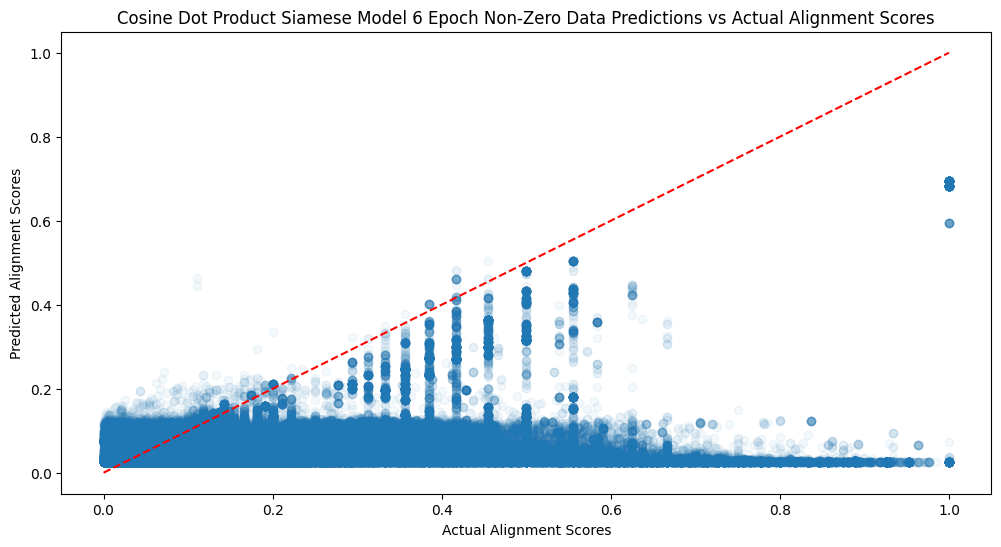
\includegraphics[scale=0.4]{Figures/ModelArchitecture/Cosine6Epoch.png}
\caption{\textbf{Scatter Plot of Cosine Similarity Siamese Model's Predictions vs. True Labels} using 80 million training samples. The diagonal line represents perfect agreement.} 
\label{fig:CosineSiameseModel}
\end{figure}

\begin{figure}[tbh!]
\centering
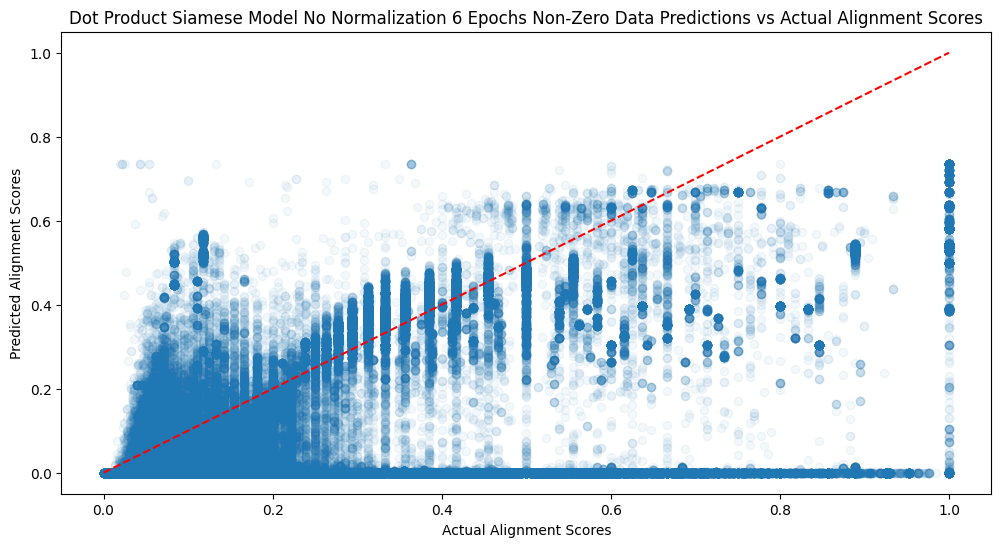
\includegraphics[scale=0.4]{Figures/ModelArchitecture/DotProdArchitecture.png}
\caption{\textbf{Scatter Plot of Dot Product Siamese Model's Predictions vs. True Labels} using 80 million training samples. The diagonal line represents perfect agreement.} 
\label{fig:NonNormSiameseModelNonNorm}
\end{figure}

Comparing figures \ref{fig:CosineSiameseModel} and \ref{fig:NonNormSiameseModelNonNorm}, it is observed that the dot product model is able to demonstrate superior generalisation and prediction compared to the cosine model. The improved results achieved by the dot product model relative to the cosine model may be attributed to the inability of cosine similarity to capture function size information. When predicting alignment scores for function merging, the actual size of functions plays a critical role in the calculation of the alignment score (\ref{METRIC:AlignmentScore}). This metric inherently depends on both the similarity of instructions and the total number of instructions in each function, making function size a key determinant.

The dot product (\ref{METRIC:DotProduct}) preserves this crucial magnitude information, allowing the model to implicitly consider both the similarity angle between functions and their relative sizes when predicting alignment scores. In contrast, cosine similarity (\ref{METRIC:CosineDistance}) normalises vector magnitudes, effectively discarding this size information. This limitation is particularly relevant when working with IR2Vec embeddings, which construct function representations through summation of the basic blocks and instructions, naturally encoding size information in vector magnitudes. The normalisation in cosine similarity causes the model to treat small functions with proportionally similar structure identically to large functions with similar structure, despite them having potentially very different alignment scores in practice, thus limiting its effectiveness for predicting alignment scores. Based on these findings, the dot product was selected as the preferred metric for the final implementation of the Siamese model.


\subsubsection{Final Model}
The fully trained and tuned dot product Siamese model demonstrated strong performance, achieving an MSE score of \textbf{0.0319} on the complete dataset and a \textbf{0.0043} on the non-zero test set.

\begin{figure}[tbh!]
\centering
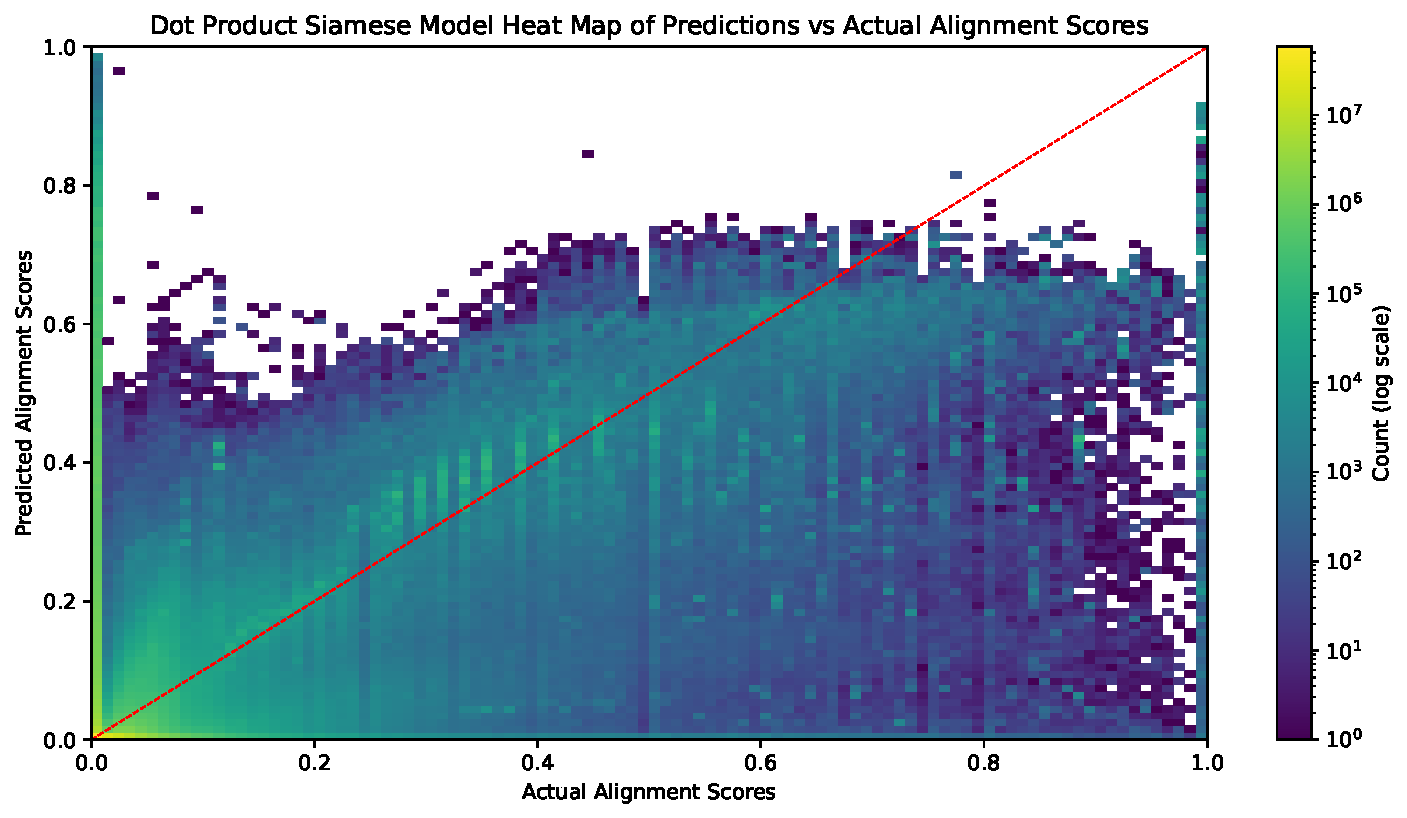
\includegraphics[scale=0.65]{Figures/Dot_Product_Siamese_Model_Heatmap.pdf}
\caption{\textbf{Frequency Heat‑map of Dot Product Siamese Model's Predictions vs. True Labels.} The colour intensity (log‑scaled count) represents the frequency in each prediction–actual score bin, and the diagonal line representing perfect agreement.} 
\label{fig:SiameseModelHeatmap}
\end{figure}

Figure \ref{fig:SiameseModelHeatmap} illustrates that the model achieves good prediction accuracy for alignment scores up to \textit{0.5}, with the majority of predictions falling near the diagonal line that represents perfect agreement. However, beyond this threshold, the model's predictions form a visible horizontal band plateauing at around \textit{0.7} in the predicted score range, making it less reliable for identifying highly aligned functions. This creates a ceiling effect where functions with true alignment scores between \textit{0.7-1.0} are consistently underestimated.

This limitation could be attributed to the imbalanced training data distribution, as evident from the colour intensity in the lower regions of the heat map, where the colour intensity indicates a significantly higher concentration of examples with lower alignment scores. Consequently, the model optimises its performance by learning to predict lower scores more frequently, which minimises the overall loss function but compromises accuracy for high-alignment cases.

\subsection{Multi-Headed Self-Attention Model Results}
The fully trained and tuned multi-headed self-attention model demonstrated exceptional performance, achieving an impressive MSE score of \textit{0.00738} across the entire testing dataset and a remarkable \textit{0.00094} for the non-zero testing dataset.


\begin{figure}[tbh!]
\centering
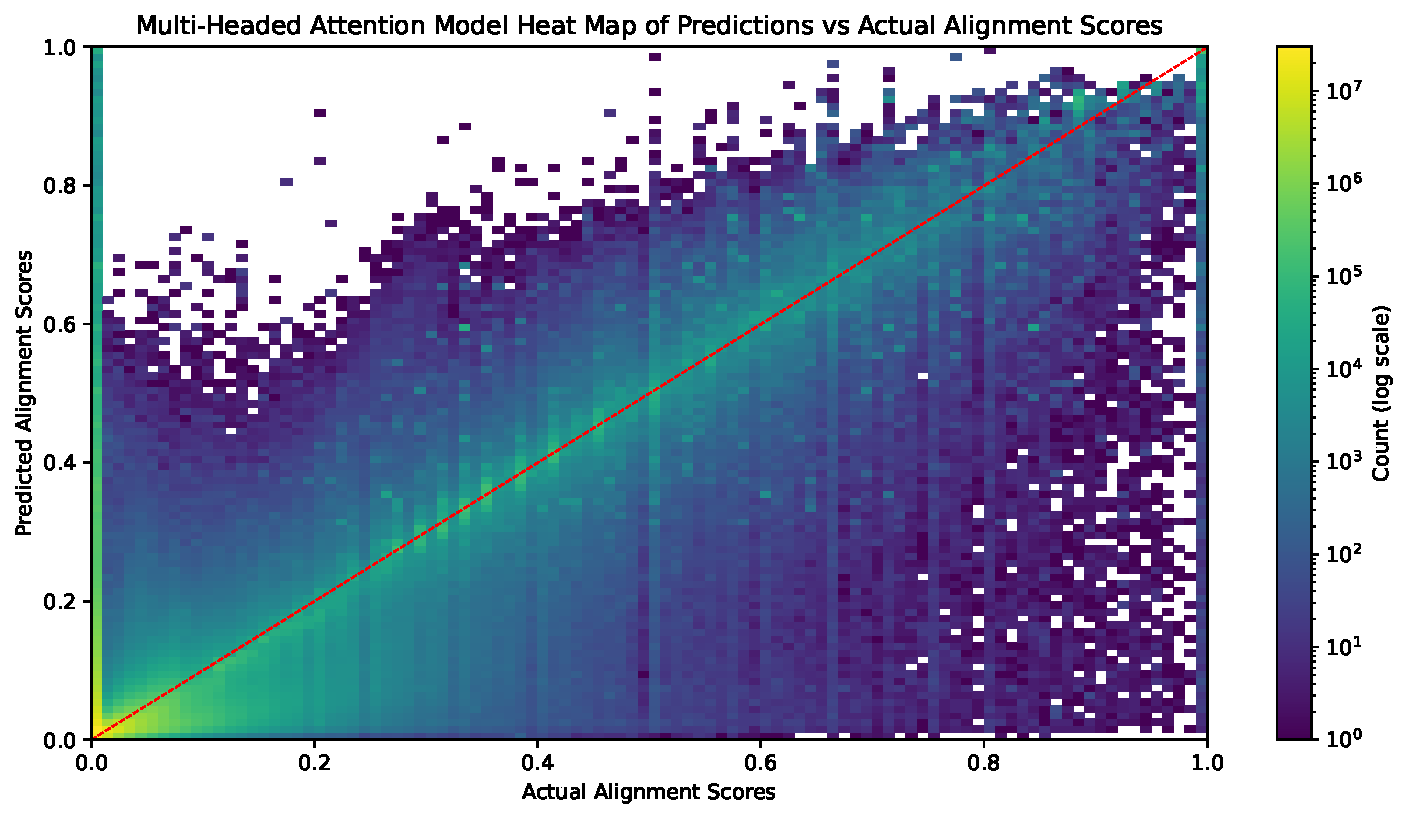
\includegraphics[scale=0.65]{Figures/Multi-Headed_Attention_Model_Heatmap.pdf}
\caption{\textbf{Frequency Heat‑map of Multi-Headed Self-Attention Model's Predictions vs. True Labels.} The colour intensity (log‑scaled count) represents the frequency in each prediction–actual score bin, and the diagonal line representing perfect agreement.} 
\label{fig:AttentionModelHeatmap}
\end{figure}

Figure \ref{fig:AttentionModelHeatmap} reveals that this model reliably predicts true alignment scores across the full spectrum of values, with most predictions closely following the diagonal line that represents perfect agreement. The heat map shows a more consistent prediction pattern along the diagonal, particularly in the 0.7-1.0 range where the Siamese model struggled. While significantly outperforming the dot product Siamese model, this attention-based architecture still exhibits a subtle bias toward under-prediction rather than over-prediction when errors occur. However, this tendency is considerably less pronounced than in the previous model, allowing for more accurate identification of highly aligned function pairs.

\subsubsection{Evaluation}
% \begin{itemize}
%     \item actual alignmnet score with 0, talk about that: This is also why we chose to use a log scale, because there are way too many 0 data points.
%     \item The dot product siamese model might miss out on potential merges because it is underpredicting the true alignment score.
%     \item predicted value does not have to be super accurate, as long as it is in the general area it is OK
% \end{itemize}

Analysis of both models reveals a common pattern in figures \ref{fig:SiameseModelHeatmap} and \ref{fig:AttentionModelHeatmap}, where samples with a true score of 0 are frequently misclassified. This observation, however, should be contextualized by the significant class imbalance in the dataset, with zero-alignment samples greatly outnumbering others as indicated by the bright yellow/green regions at the origin of both heat maps. Notably, for both models, prediction errors decrease as the predicted values move away from 0, indicating robust discrimination capabilities even with imbalanced training data.

When directly comparing performance, the multi-headed self-attention model demonstrates substantially superior prediction accuracy across the entire alignment score range. This improvement is particularly significant for higher alignment scores, where the Siamese model's plateauing effect limits its utility. The visual difference between the two heat maps is striking, the attention model shows a much more defined diagonal pattern throughout the entire range, especially above \textit{0.7}. The practical implication of implementing the Siamese model in a production environment may result in missed opportunities for merging highly aligned function pairs due to systematic under-prediction, potentially reducing the overall effectiveness of the system. Conversely, the attention model's more balanced error distribution makes it a more reliable choice for accurately identifying candidates for function merging across the full spectrum of alignment scores.

The comparative analysis reveals that the attention architecture demonstrates is more forgiving towards data imbalance, maintaining high performance even with minimal pre-processing techniques. On the other hand, the Siamese architecture exhibits clear limitations when trained on skewed distributions, suggesting that it would benefit from more sophisticated preprocessing approaches. This fundamental difference in how each architecture handles class imbalance represents an important consideration for deployment scenarios where balanced training data cannot be guaranteed.

\section{Quality of Merging Predictions}
To assess and compare the quality of the merging decisions between F3M and the ML approach, function merging was performed on the Spec2006 and Spec2017 benchmarks to collect performance data. This evaluation employs three metrics in combination to quantify the quality of the predictions: the number of total merges made, the number of valid merges and the number of profitable merges.

For each function, the system identifies another function with the highest alignment score as a potential merging candidate. If this score exceeds a pre-determined threshold, the two functions are considered for merging. This thresholding strategy aims to reduce the compile time by eliminating low-potential merging attempts that would likely prove unprofitable. The merging process yields two outcomes, whether it is possible to merge the functions (\textbf{validity}) and if valid, whether the merged function is \textbf{profitable}. 

The evaluation uses three plots to visualise the quality of the predictions:
\begin{itemize}
    \item The total number of attempted merges
    \item The percentage of merges that are valid
    \item The percentage of valid merges that are profitable
\end{itemize}
These percentages are calculated using equations \ref{METRIC:ValidPercentage} and \ref{METRIC:ValidProfitablePercentage} respectively. The evaluation assesses the quality of the predictions across three thresholds: 0.4, 0.5, and 0.6. 

\begin{equation} \label{METRIC:ValidPercentage}
    Valid\ Percentage(\%) =\frac{No.\ of\ Valid\ Merges}{Total\ No.\ of\ Attempted\ Merges}
\end{equation}

\begin{equation} \label{METRIC:ValidProfitablePercentage}
    Valid\ Profitable\ Percentage (\%)=\frac{No.\ of\ Profitable\ Merges}{No.\ of\ Valid\ Merges}
\end{equation}


\subsection{Number of Attempted Merges}
Figure \ref{fig:AttemptedMerges} collectively show the number of attempted function merges for F3M, dot product model prediction approach and the attention model prediction approach across all prediction threshold values.

\begin{figure}[tbh!]
    \centering
    \begin{subfigure}{\textwidth}
        \centering
        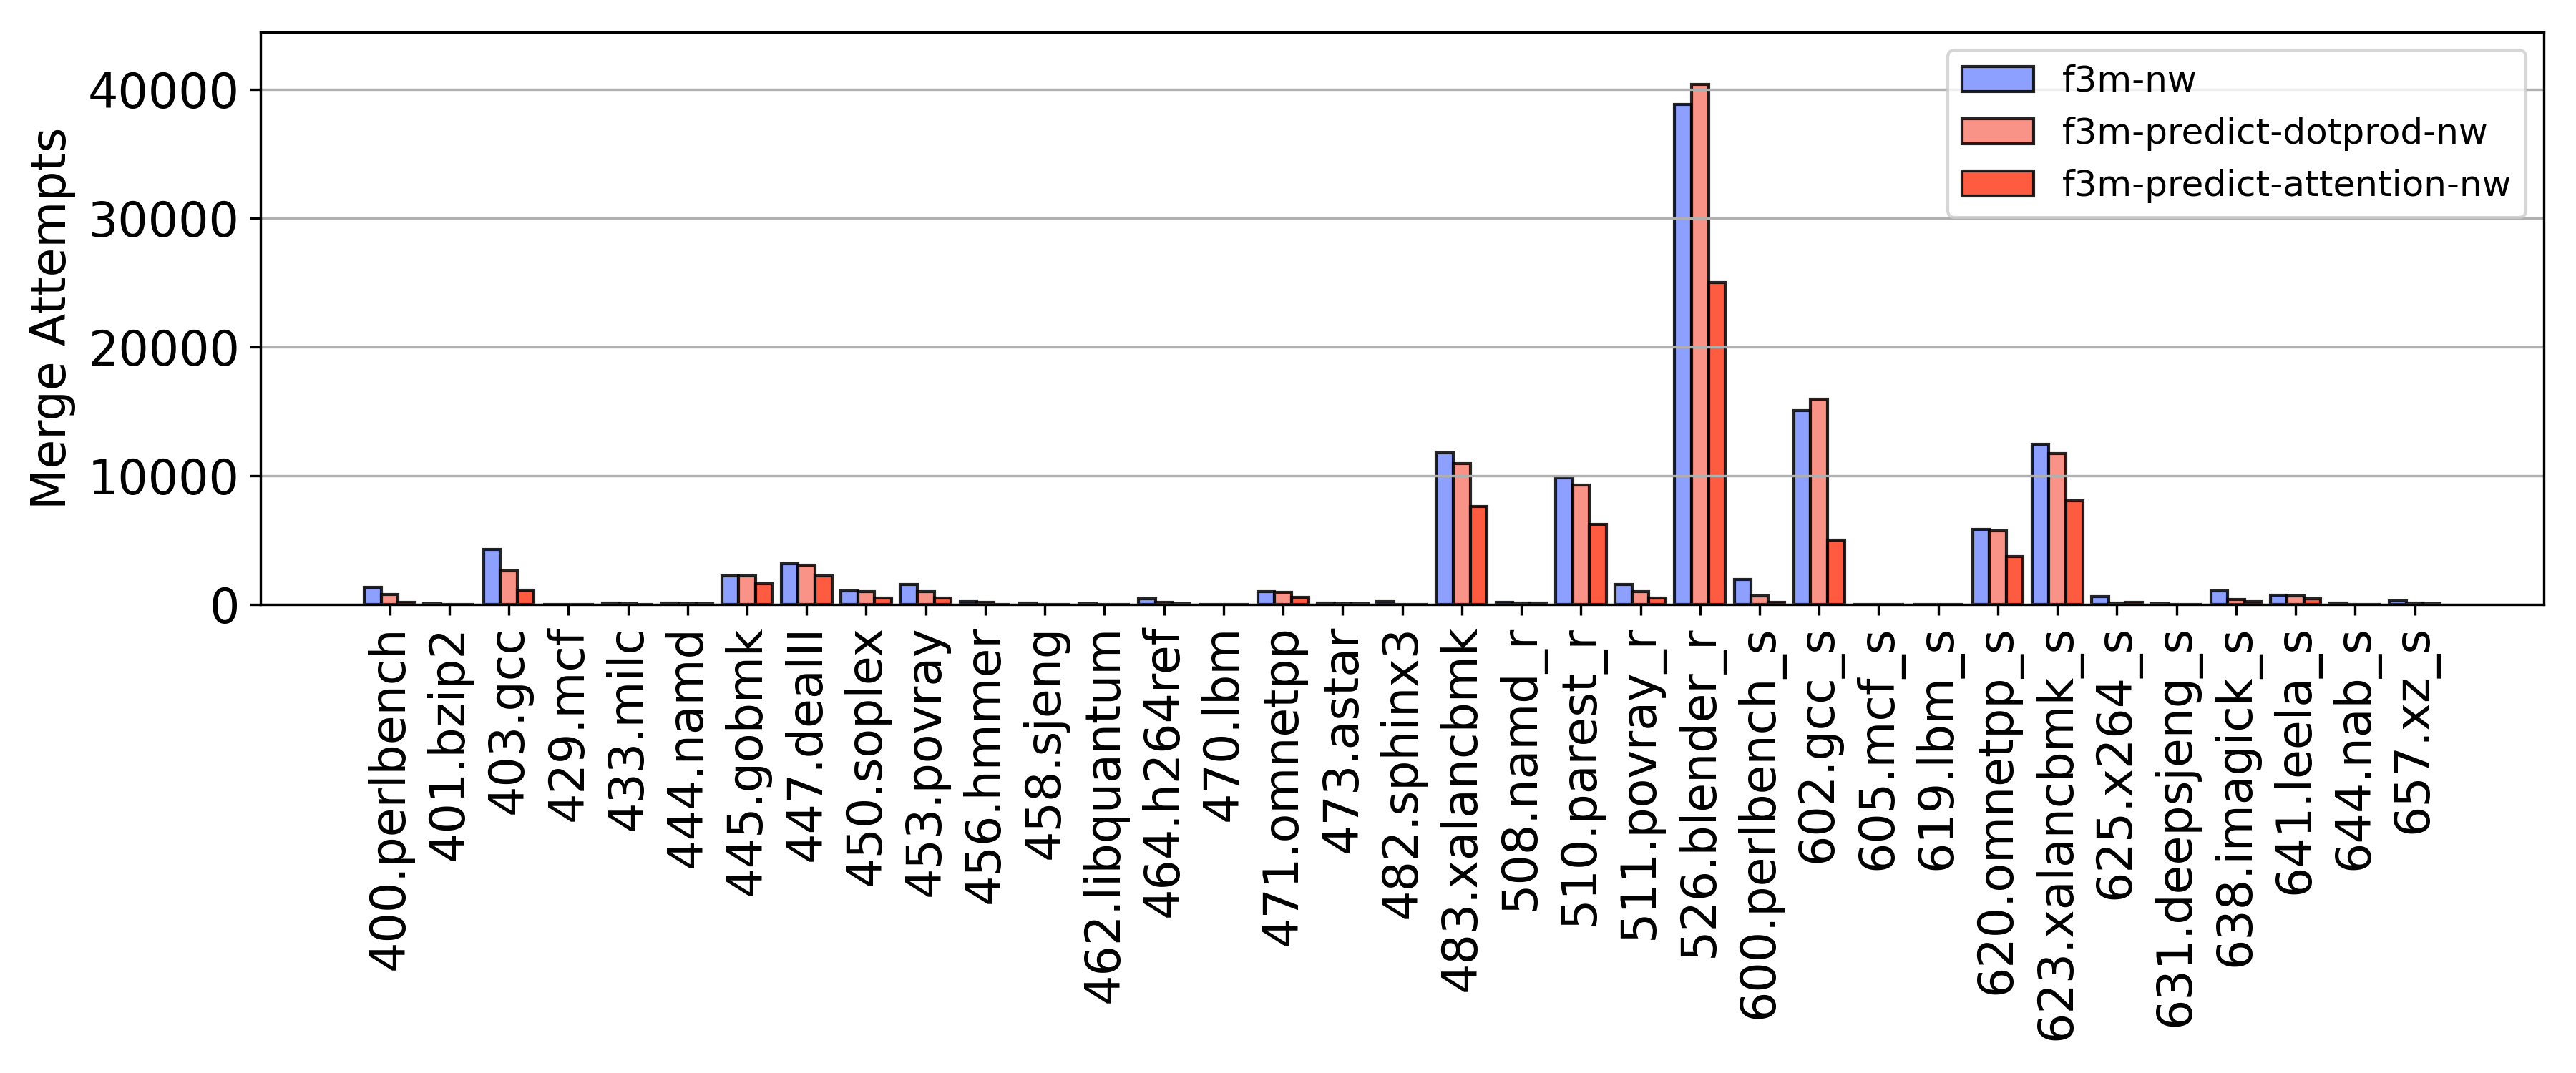
\includegraphics[scale=0.47]{Figures/Valid_Merging_Predictions/0.4_MergeAttempts.png}
        \caption{\textbf{Number of Attempted Merges (\textbf{0.4} Threshold)}} 
        \label{fig:0.4AttemptedMerges}
    \end{subfigure}
    \begin{subfigure}{\textwidth}
        \centering
        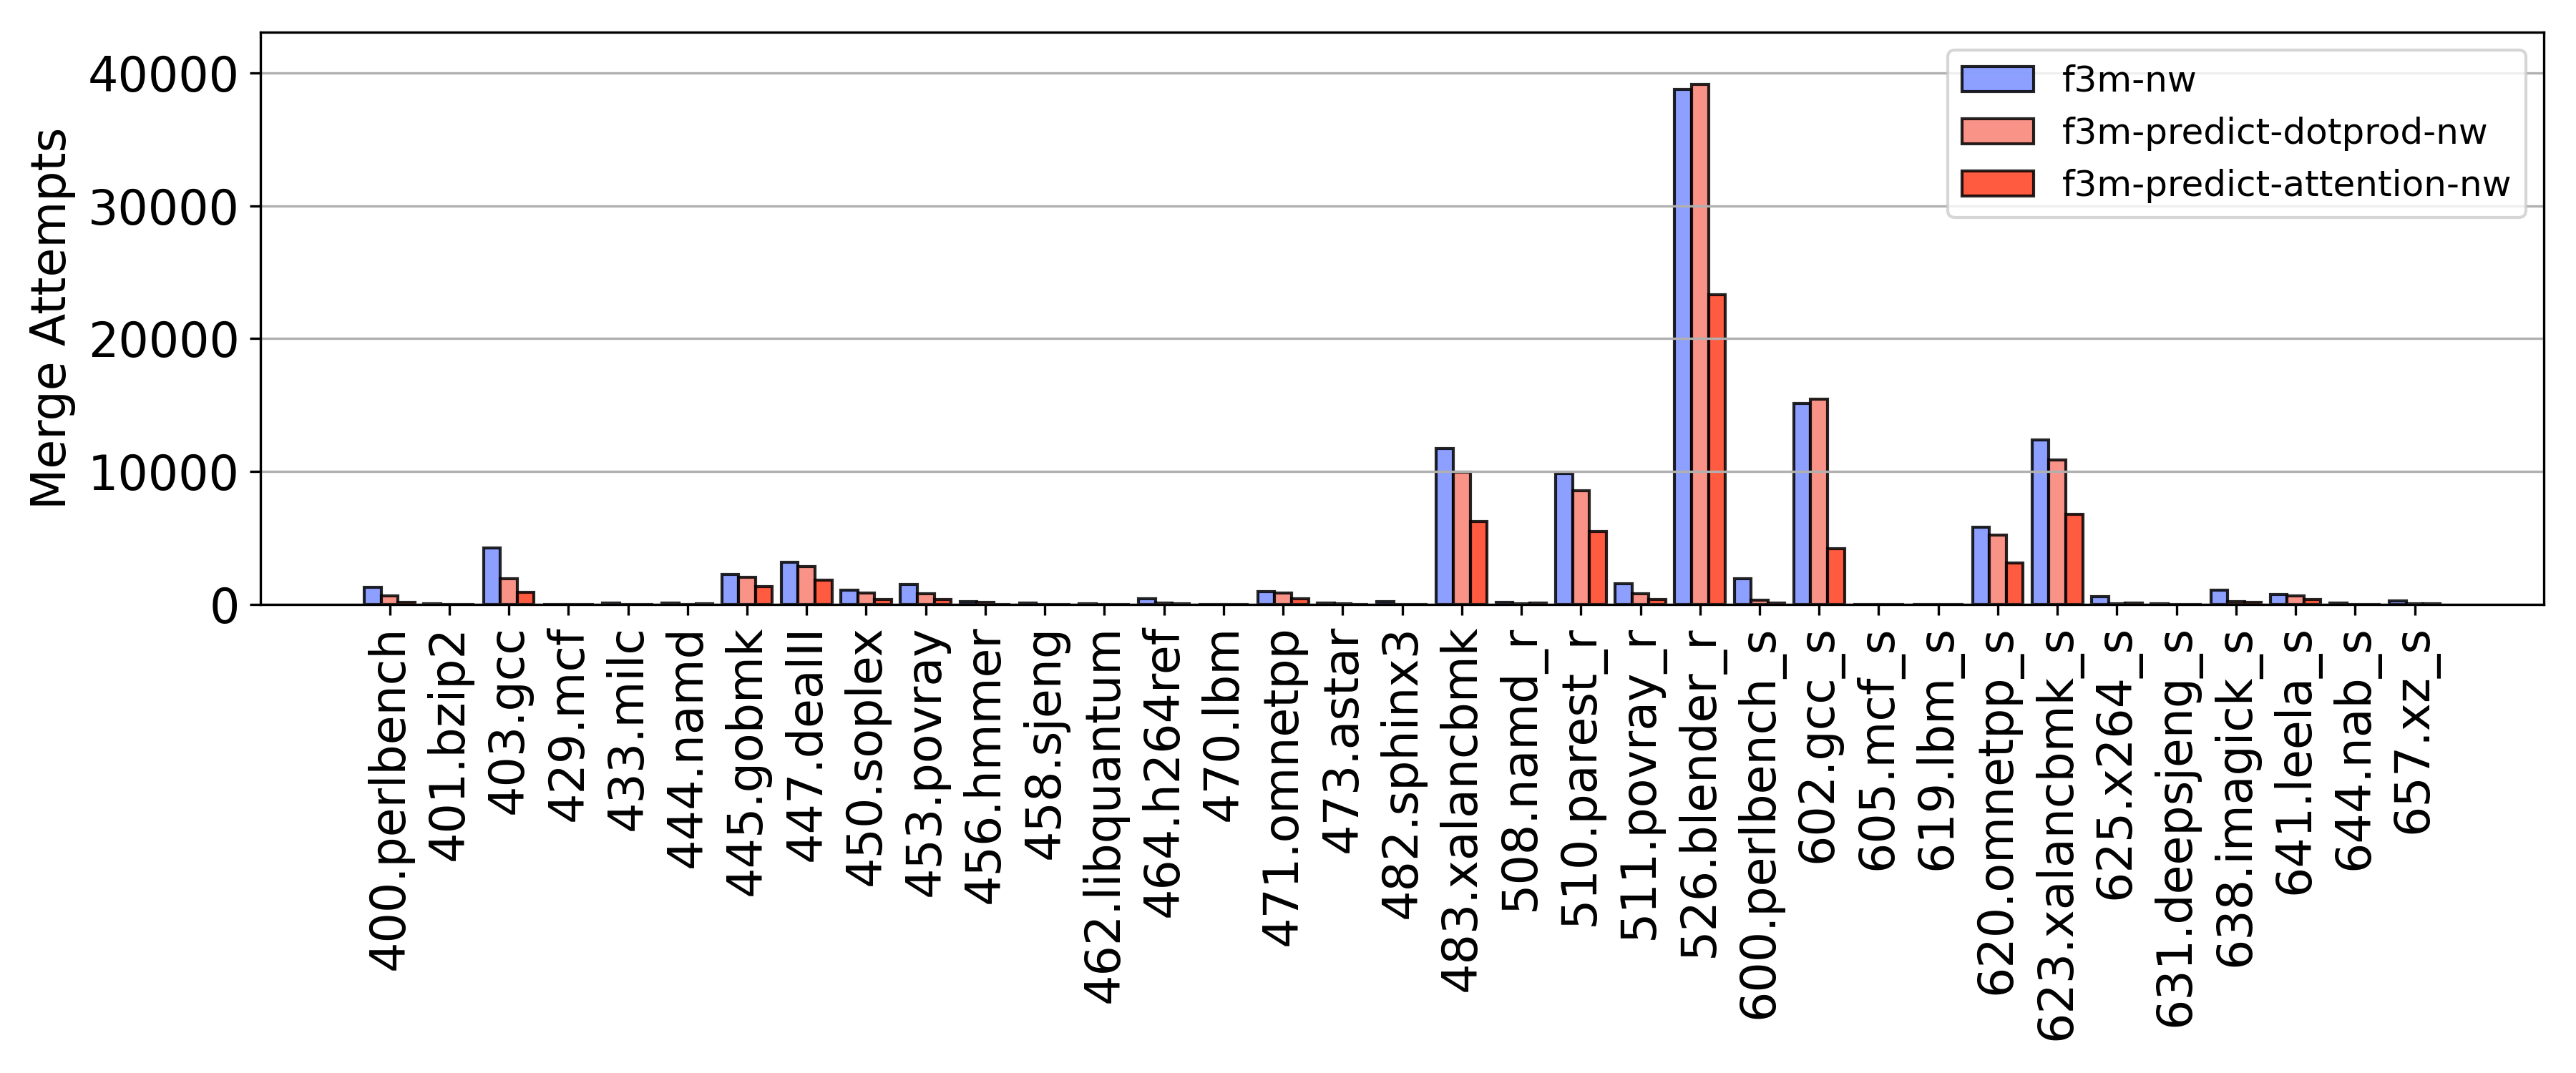
\includegraphics[scale=0.47]{Figures/Valid_Merging_Predictions/0.5_MergeAttempts.png}
        \caption{\textbf{Number of Attempted Merges (\textbf{0.5} Threshold)}} 
        \label{fig:0.5AttemptedMerges}
    \end{subfigure}
    \begin{subfigure}{\textwidth}
    \centering
        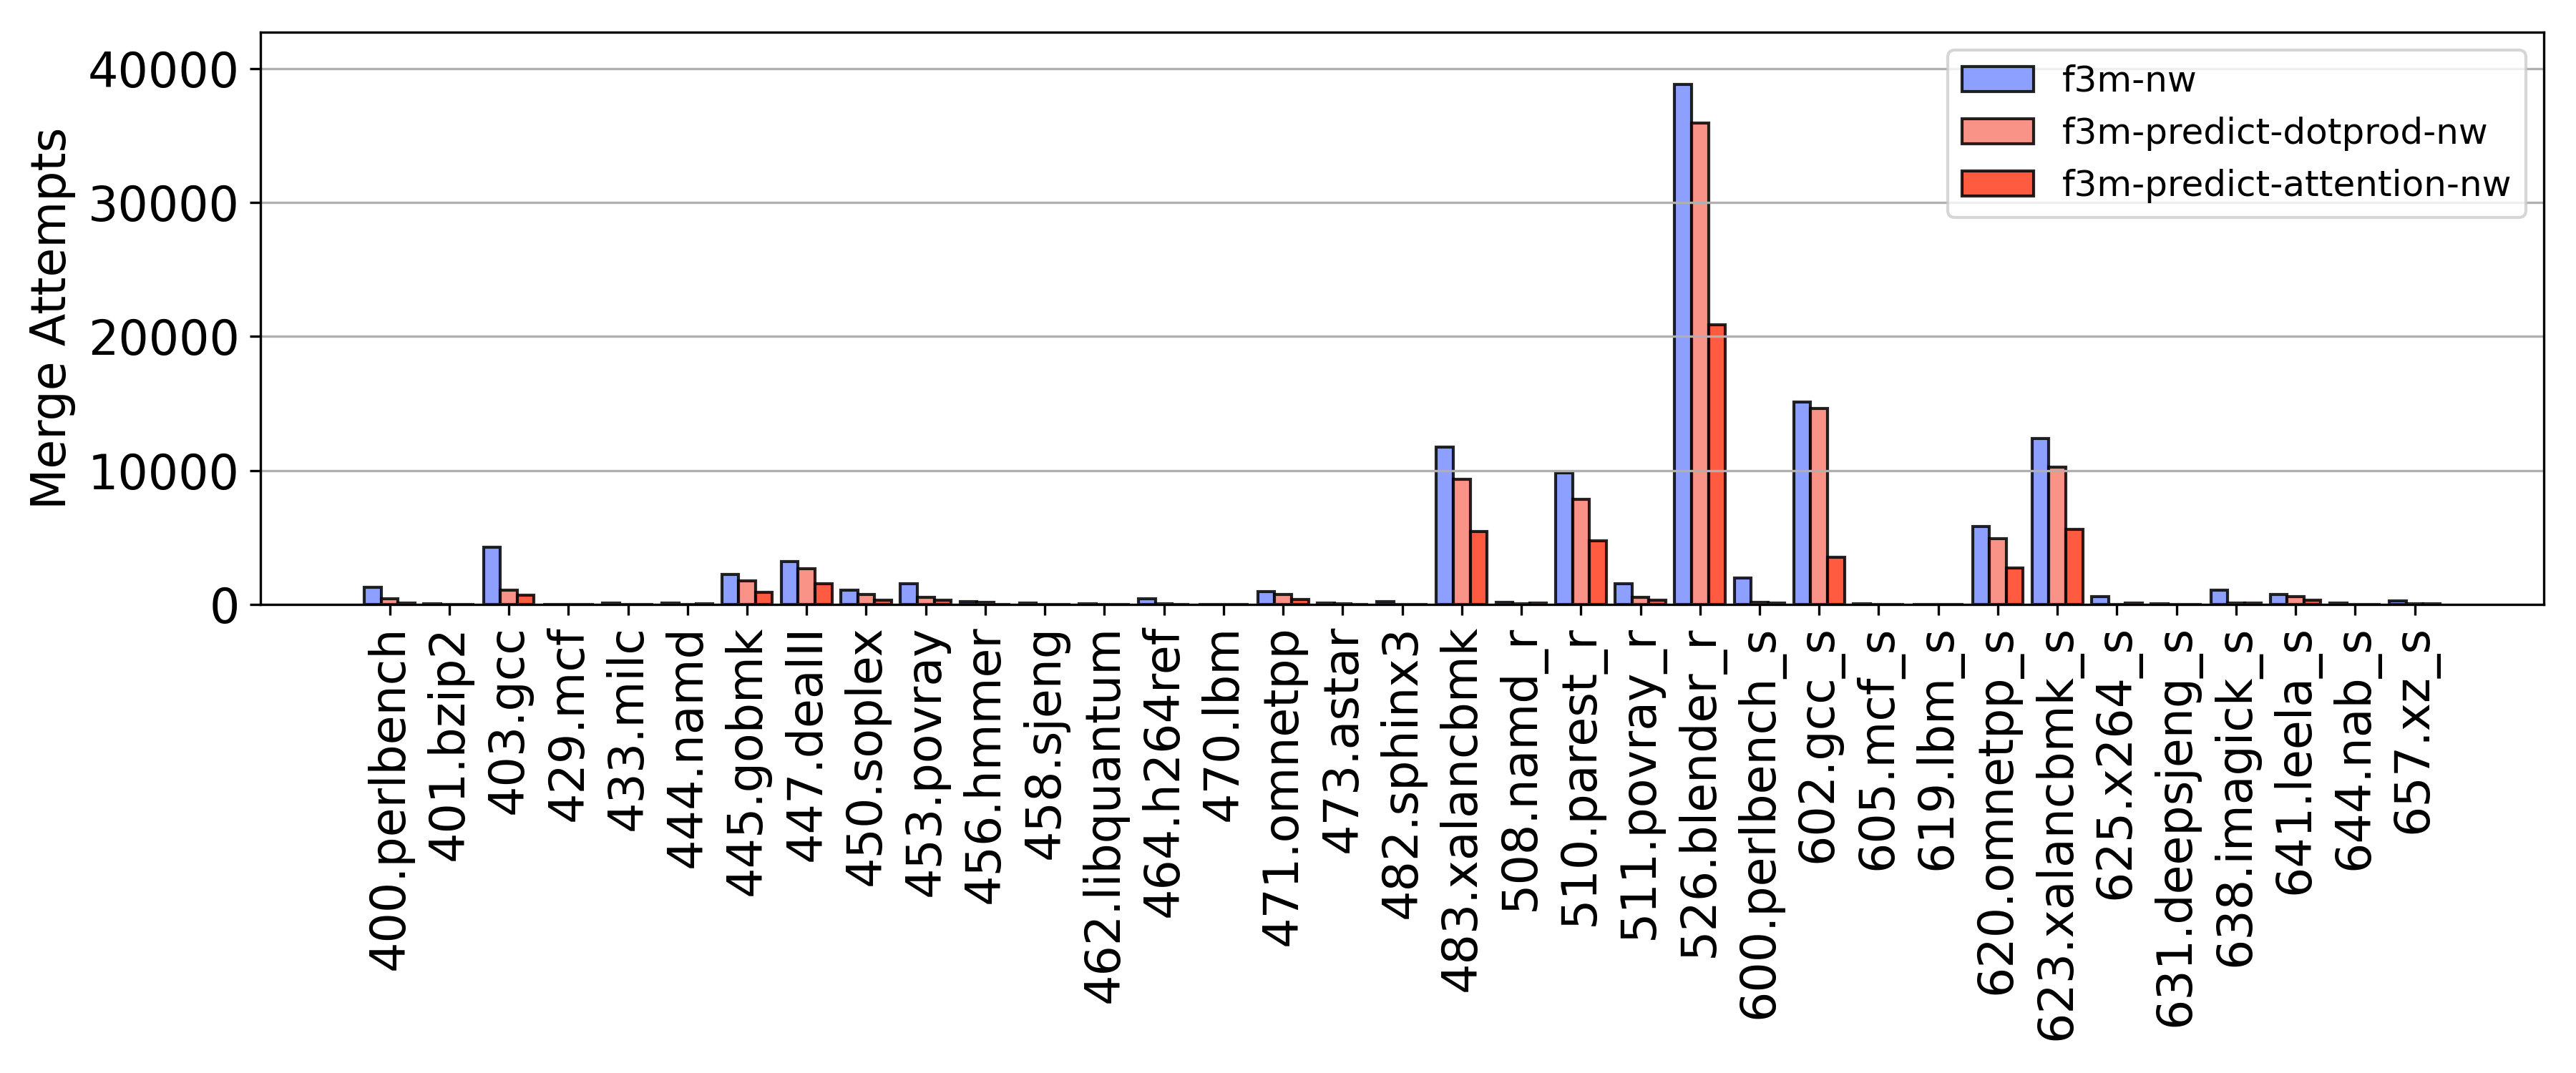
\includegraphics[scale=0.47]{Figures/Valid_Merging_Predictions/0.6_MergeAttempts.png}
        \caption{\textbf{Number of Attempted Merges (\textbf{0.6} Threshold)}} 
        \label{fig:0.6AttemptedMerges}
    \end{subfigure}

    \caption{\textbf{Number of Attempted Merges} for each threshold.} 
    \label{fig:AttemptedMerges}
\end{figure}

The benchmark \textit{526.blender\_r} exhibits the most merging attempts, more than double that of the next highest benchmark, while \textit{429.mcf} and \textit{605.mcf\_s} have the least amount of attempted merges. This disparity indicates that blender contains a lot of function candidates for function merging operations, while mcf offers a limited number of options, restricting the potential for merging due to the lack of available pairs.

As the threshold increases, both predictive models demonstrate an inverse correlation with the number of merge attempts as expected. This effect is particularly pronounced in the dot product model, which initially attempts more merges than F3M in some cases at a threshold of 0.4, matches F3M generally at 0.5, and finally predicts fewer function merges at a threshold of 0.6. In contrast, the attention model consistently predicts significantly fewer suitable functions to merge than the other two implementations across the whole benchmark suite, with some cases such as \textit{602.gcc\_s} showing more than 50\% fewer attempts.



\subsection{Validity of Merging Attempts}
Figure \ref{fig:Valid} plot the ratio of the attempted merges that were able to produce a merged function (validity) for each prediction threshold. This validity metric allows us to normalise the data against the varying attempted merges and compare performance across the implementations.

\begin{figure}[tbh!]
    \centering
    \begin{subfigure}{\textwidth}
        \centering
        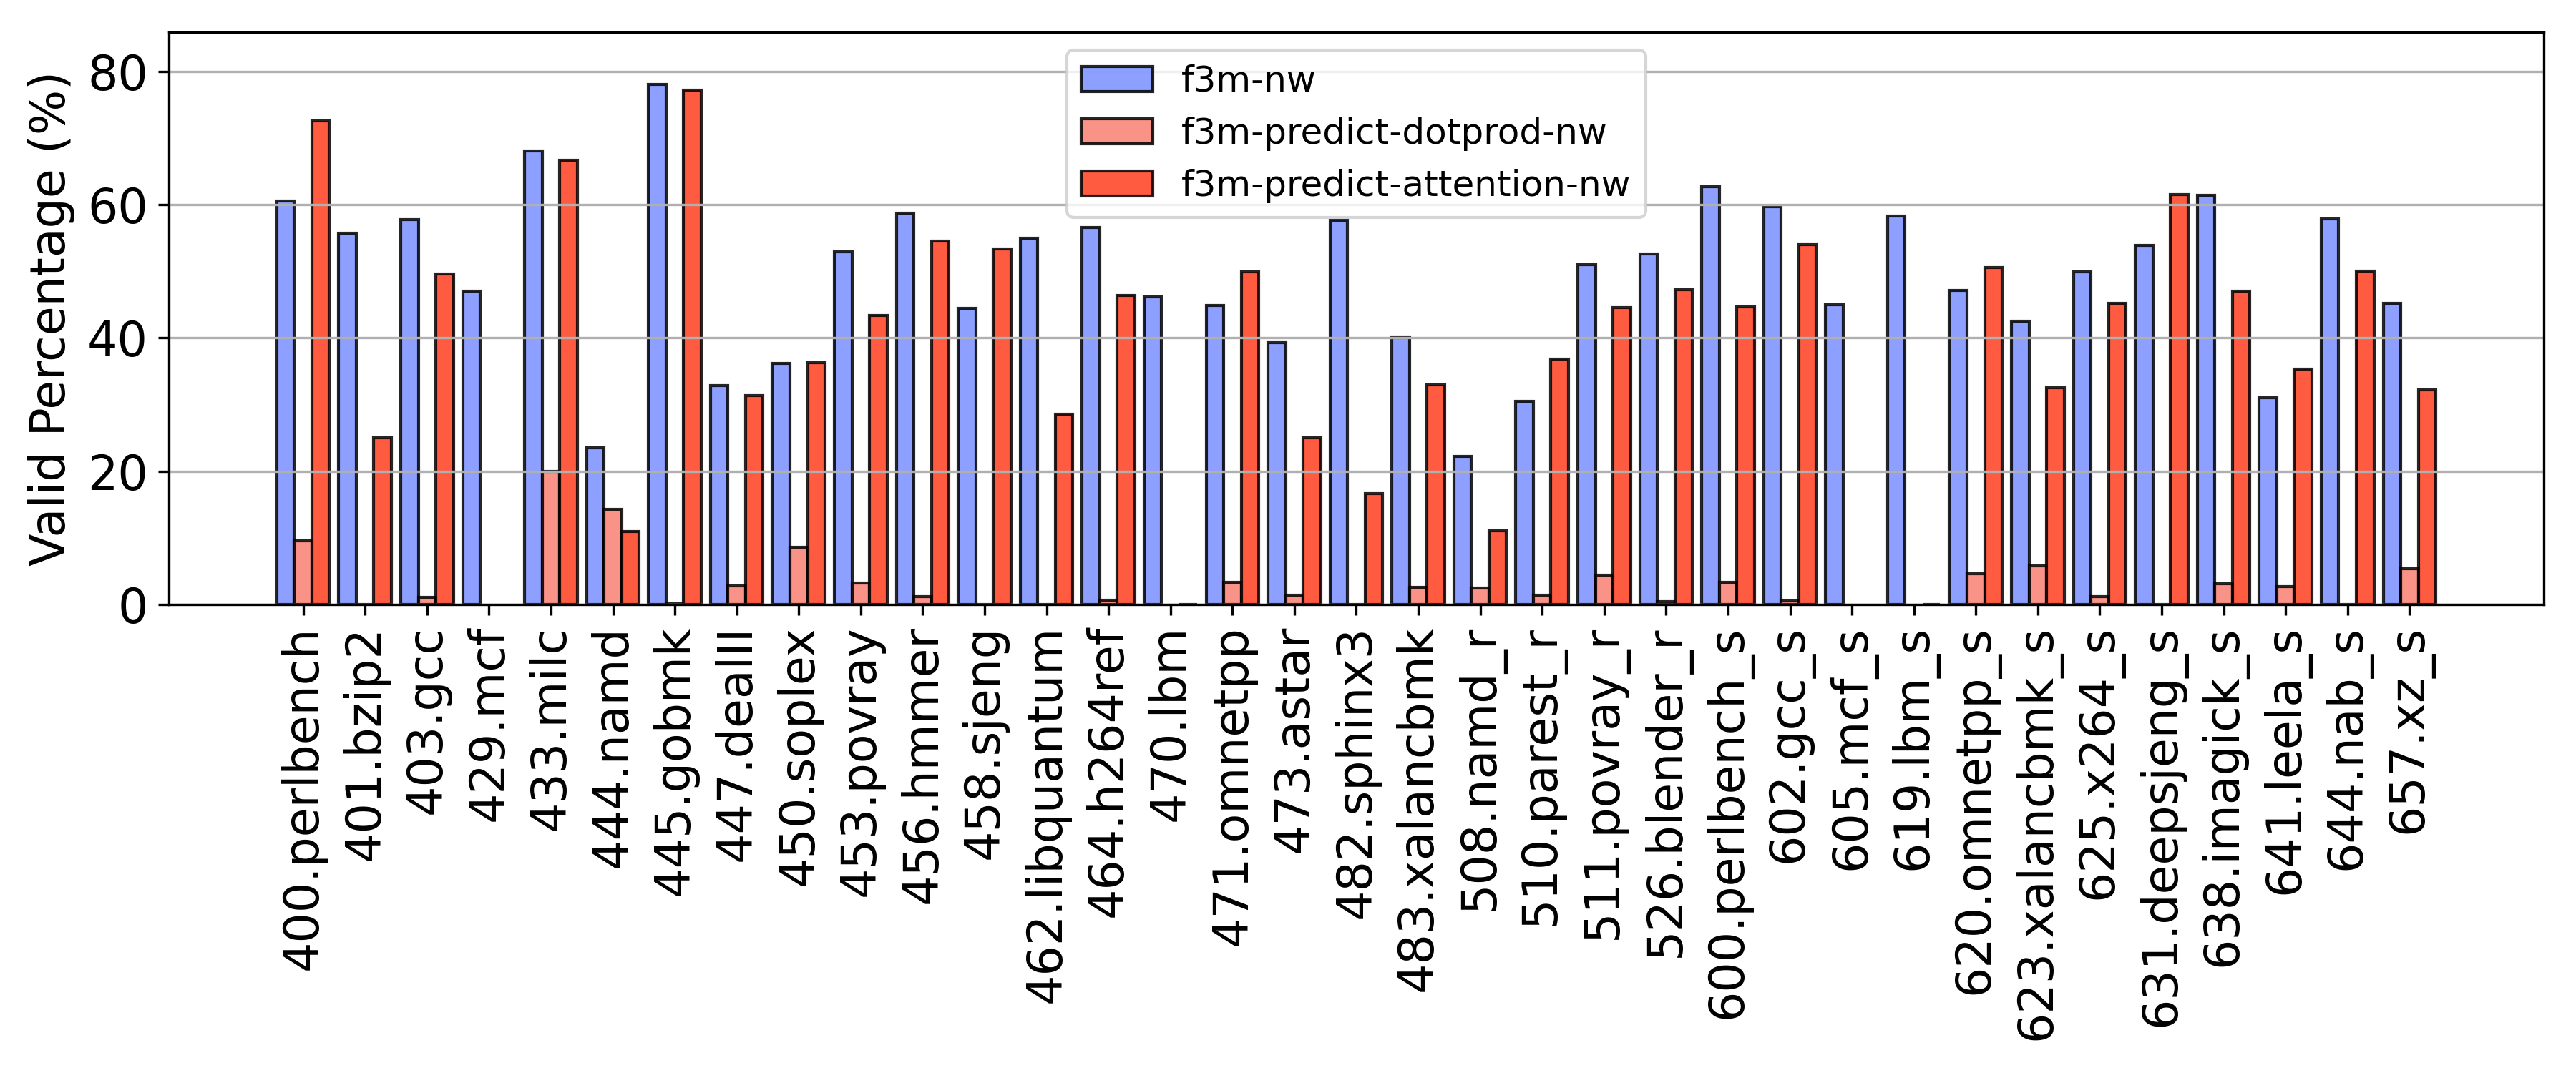
\includegraphics[scale=0.47]{Figures/Valid_Merging_Predictions/0.4_ValidPercentage.png}
        \caption{\textbf{Ratio of Valid Merges (\textbf{0.4} Threshold)}} 
        \label{fig:0.4Valid}
    \end{subfigure}
    \begin{subfigure}{\textwidth}
        \centering
        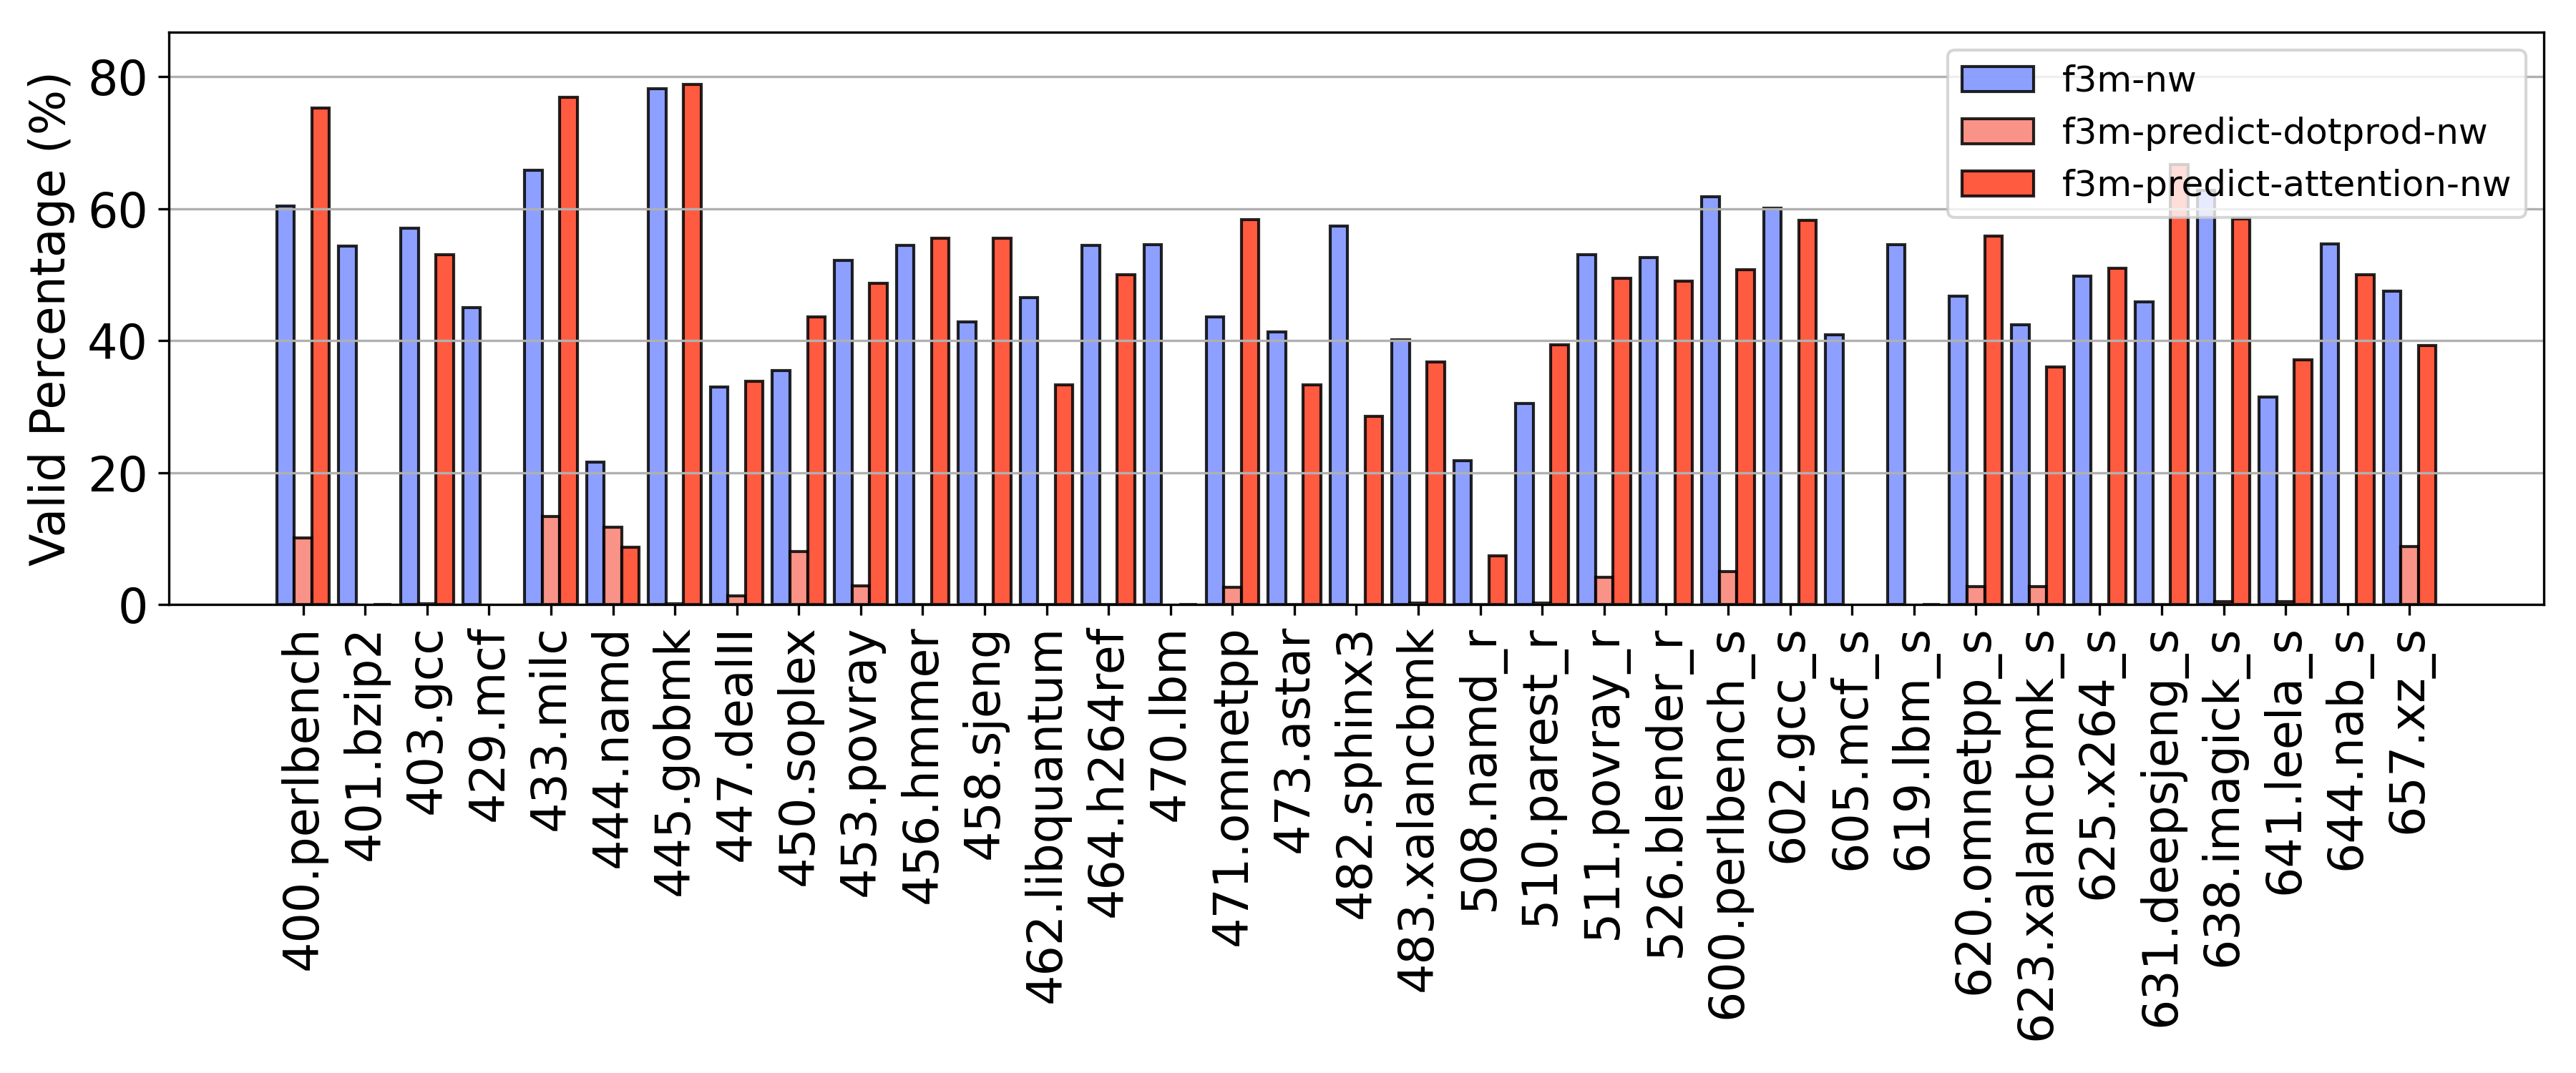
\includegraphics[scale=0.47]{Figures/Valid_Merging_Predictions/0.5_ValidPercentage.png}
        \caption{\textbf{Ratio of Valid Merges (\textbf{0.5} Threshold)}} 
        \label{fig:0.5Valid}
    \end{subfigure}
    \begin{subfigure}{\textwidth}
    \centering
        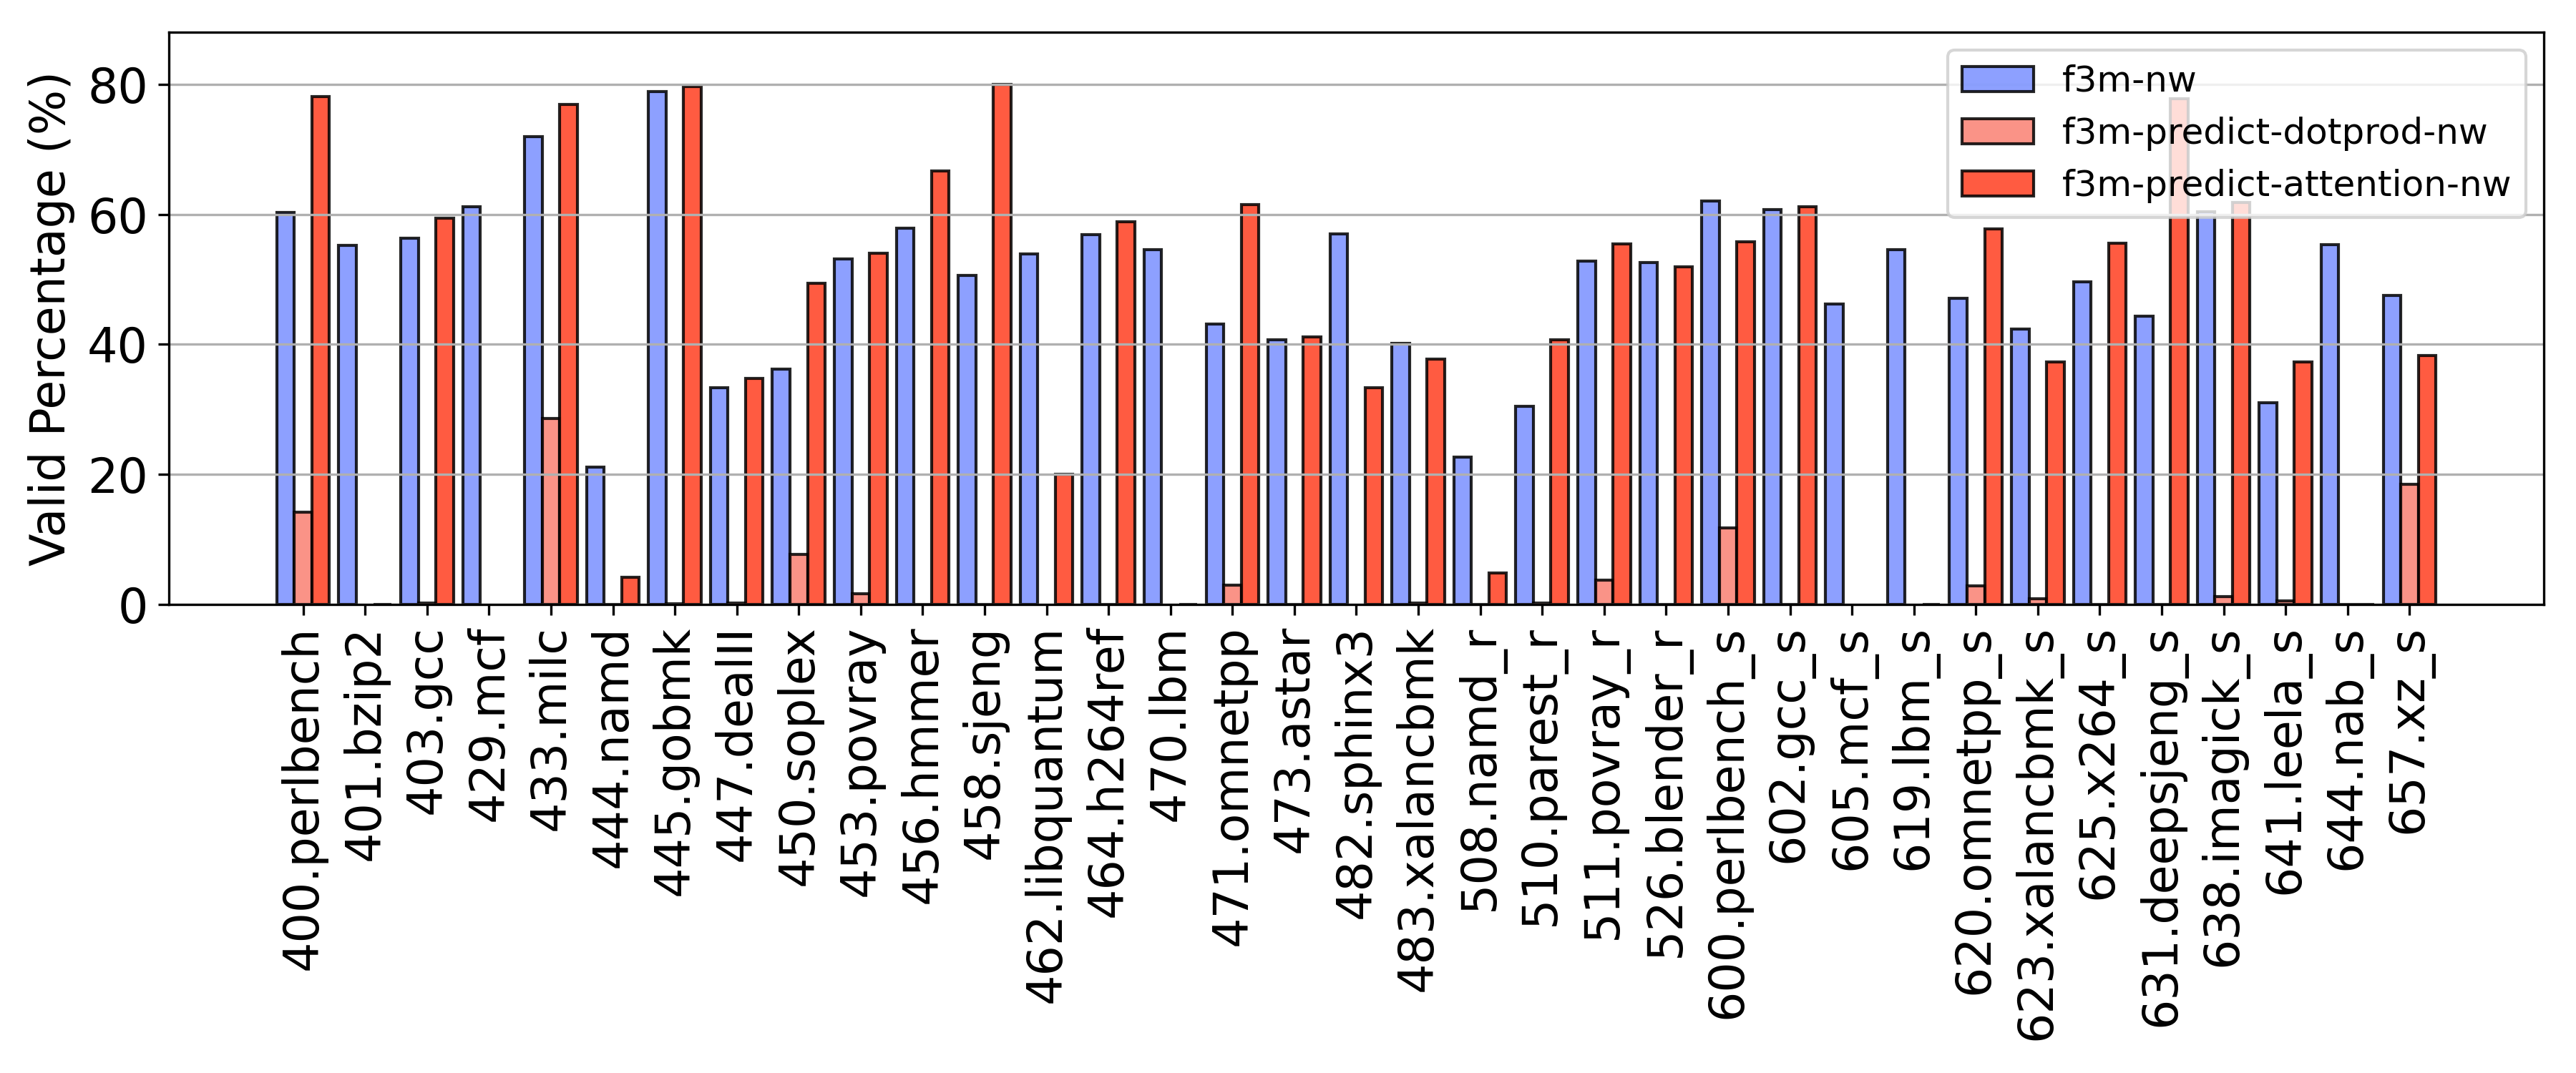
\includegraphics[scale=0.47]{Figures/Valid_Merging_Predictions/0.6_ValidPercentage.png}
        \caption{\textbf{Ratio of Valid Merges (\textbf{0.6} Threshold)}} 
        \label{fig:0.6Valid}
    \end{subfigure}

    \caption{\textbf{Percentage of Attempted Merges that are Valid.} This graph shows the proportion of merge attempts resulting in valid function pairs, calculated using equation \ref{METRIC:ValidPercentage}.} 
    \label{fig:Valid}
\end{figure}

Looking at all three figures, we can quickly determine that the dot product approach fails to reliably predict valid function pairs that are suitable for merging regardless of the threshold value, struggling to break the 10\% mark in most cases. The attention model, by contrast, demonstrates considerably better ability to pick out function pairs that produce valid merges, showing an inverse relationship between the threshold and the validity percentage. This improvement is likely due to higher thresholds filtering out function pairs that the model is not confident about. At a threshold of 0.4, the attention model underperforms compared to F3M in most benchmarks (only 7 out of 35 meeting or exceeding F3M), while at 0.5 the model approximately matches F3M's performance on average (13 out of 35 benchmarks). At 0.6, the attention model outperforms F3M in the majority of cases (20 out of 35 benchmarks).

\subsection{Profitability of Valid Merges}
Finally, figure \ref{fig:ValidProfitable} graphs the percentage of valid merges that produced a profitable merged function. Profitability is determined when the estimated size of the newly merged function is smaller than the sum of the estimated sizes of the original function pair.

\begin{figure}[tbh!]
    \centering
    \begin{subfigure}{\textwidth}
        \centering
        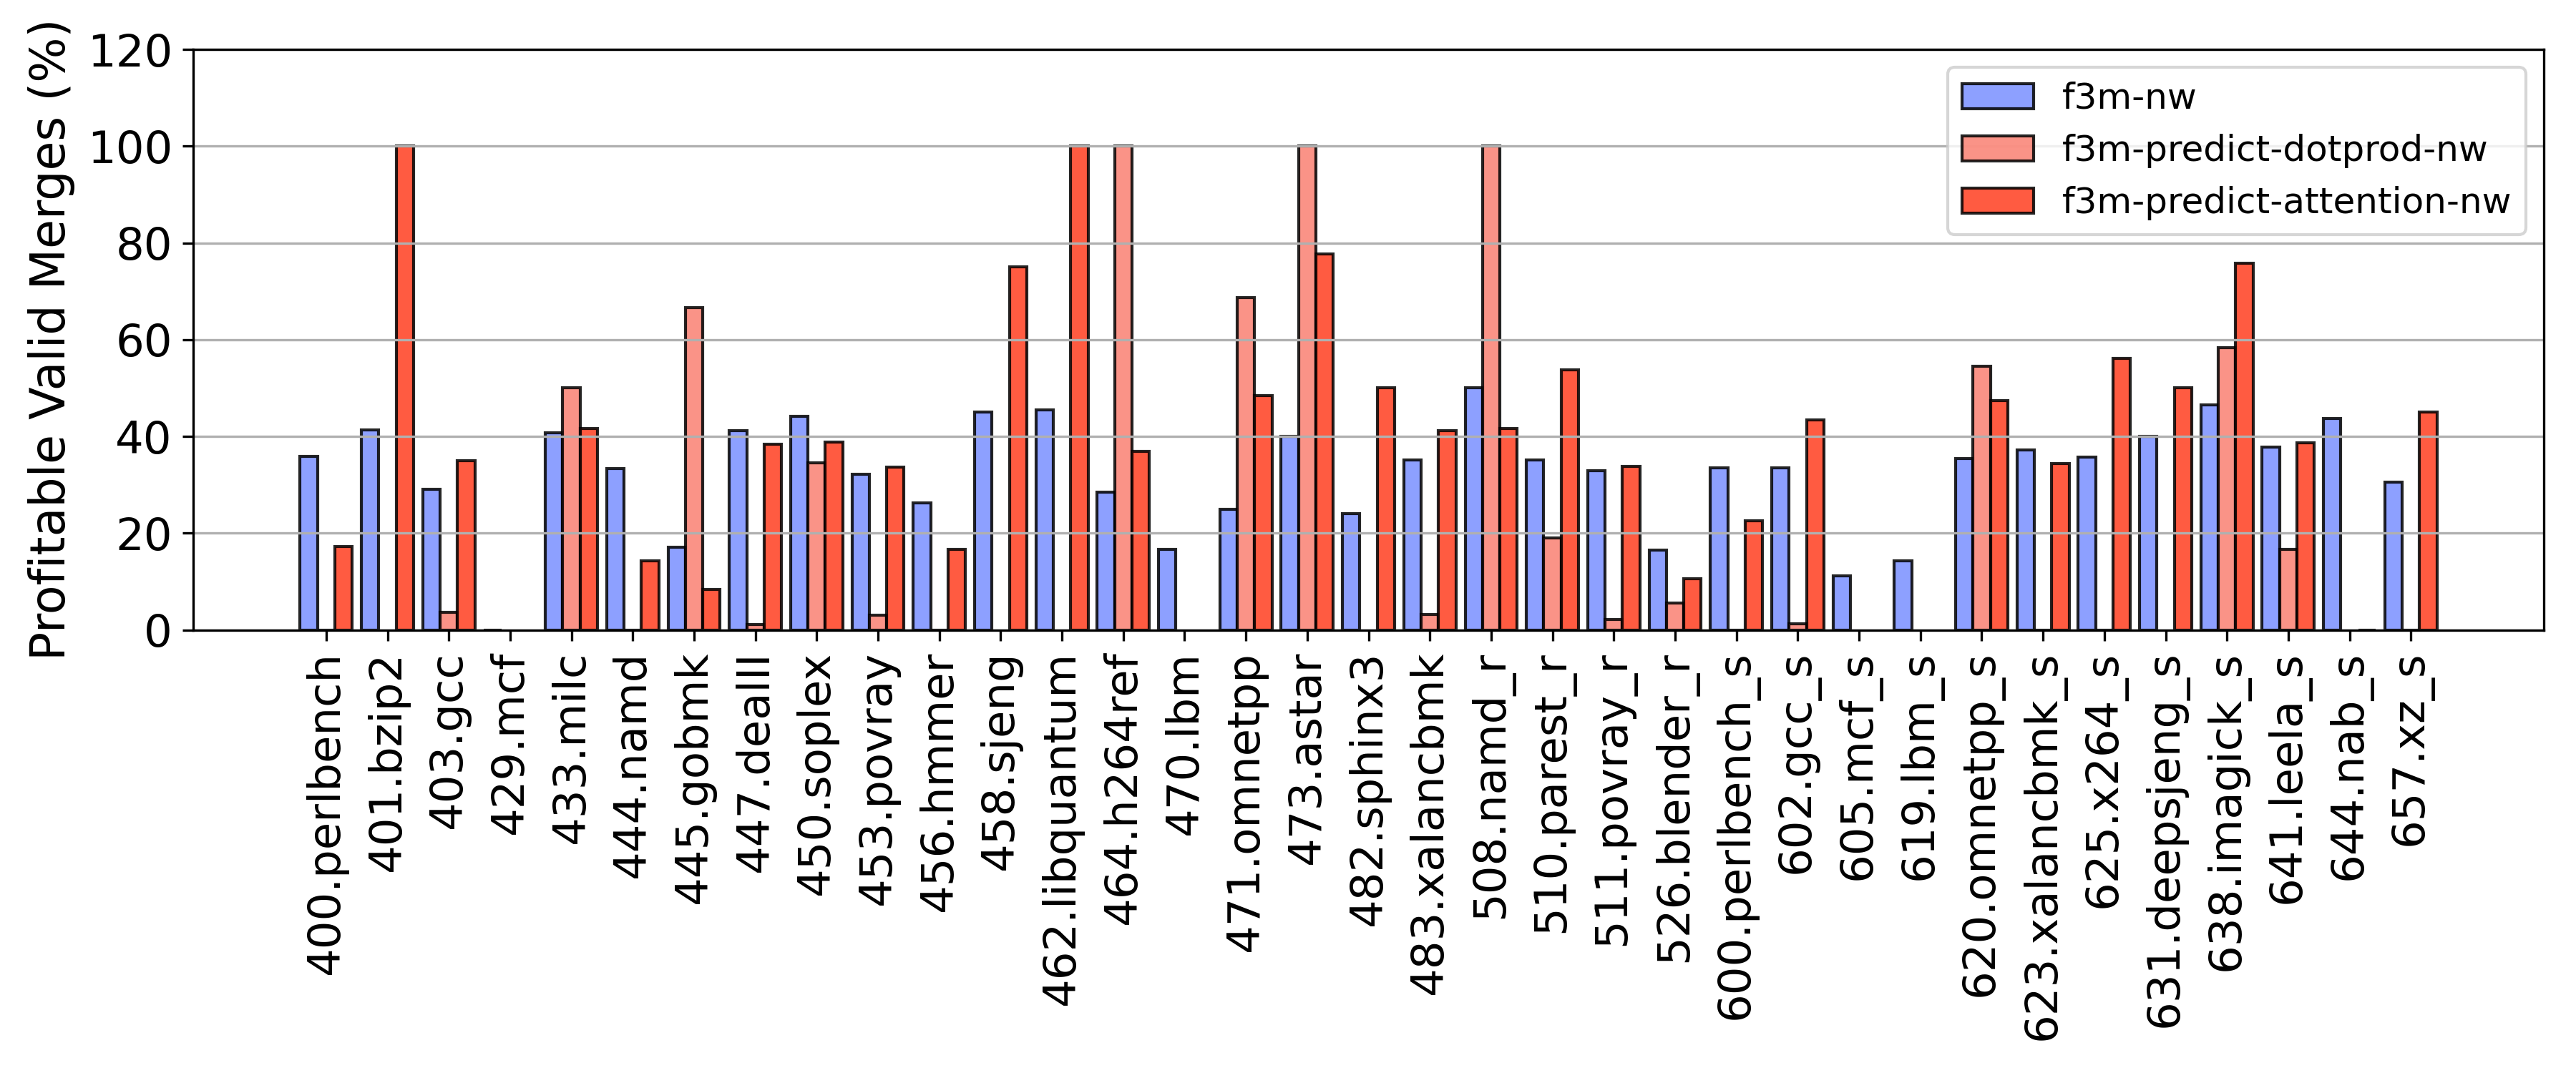
\includegraphics[scale=0.47]{Figures/Valid_Merging_Predictions/0.4_ValidProfitablePercentage.png}
        \caption{\textbf{Profitable Valid Merges (\textbf{0.4} Threshold)}} 
        \label{fig:0.4ValidProfitable}
    \end{subfigure}
    \begin{subfigure}{\textwidth}
        \centering
        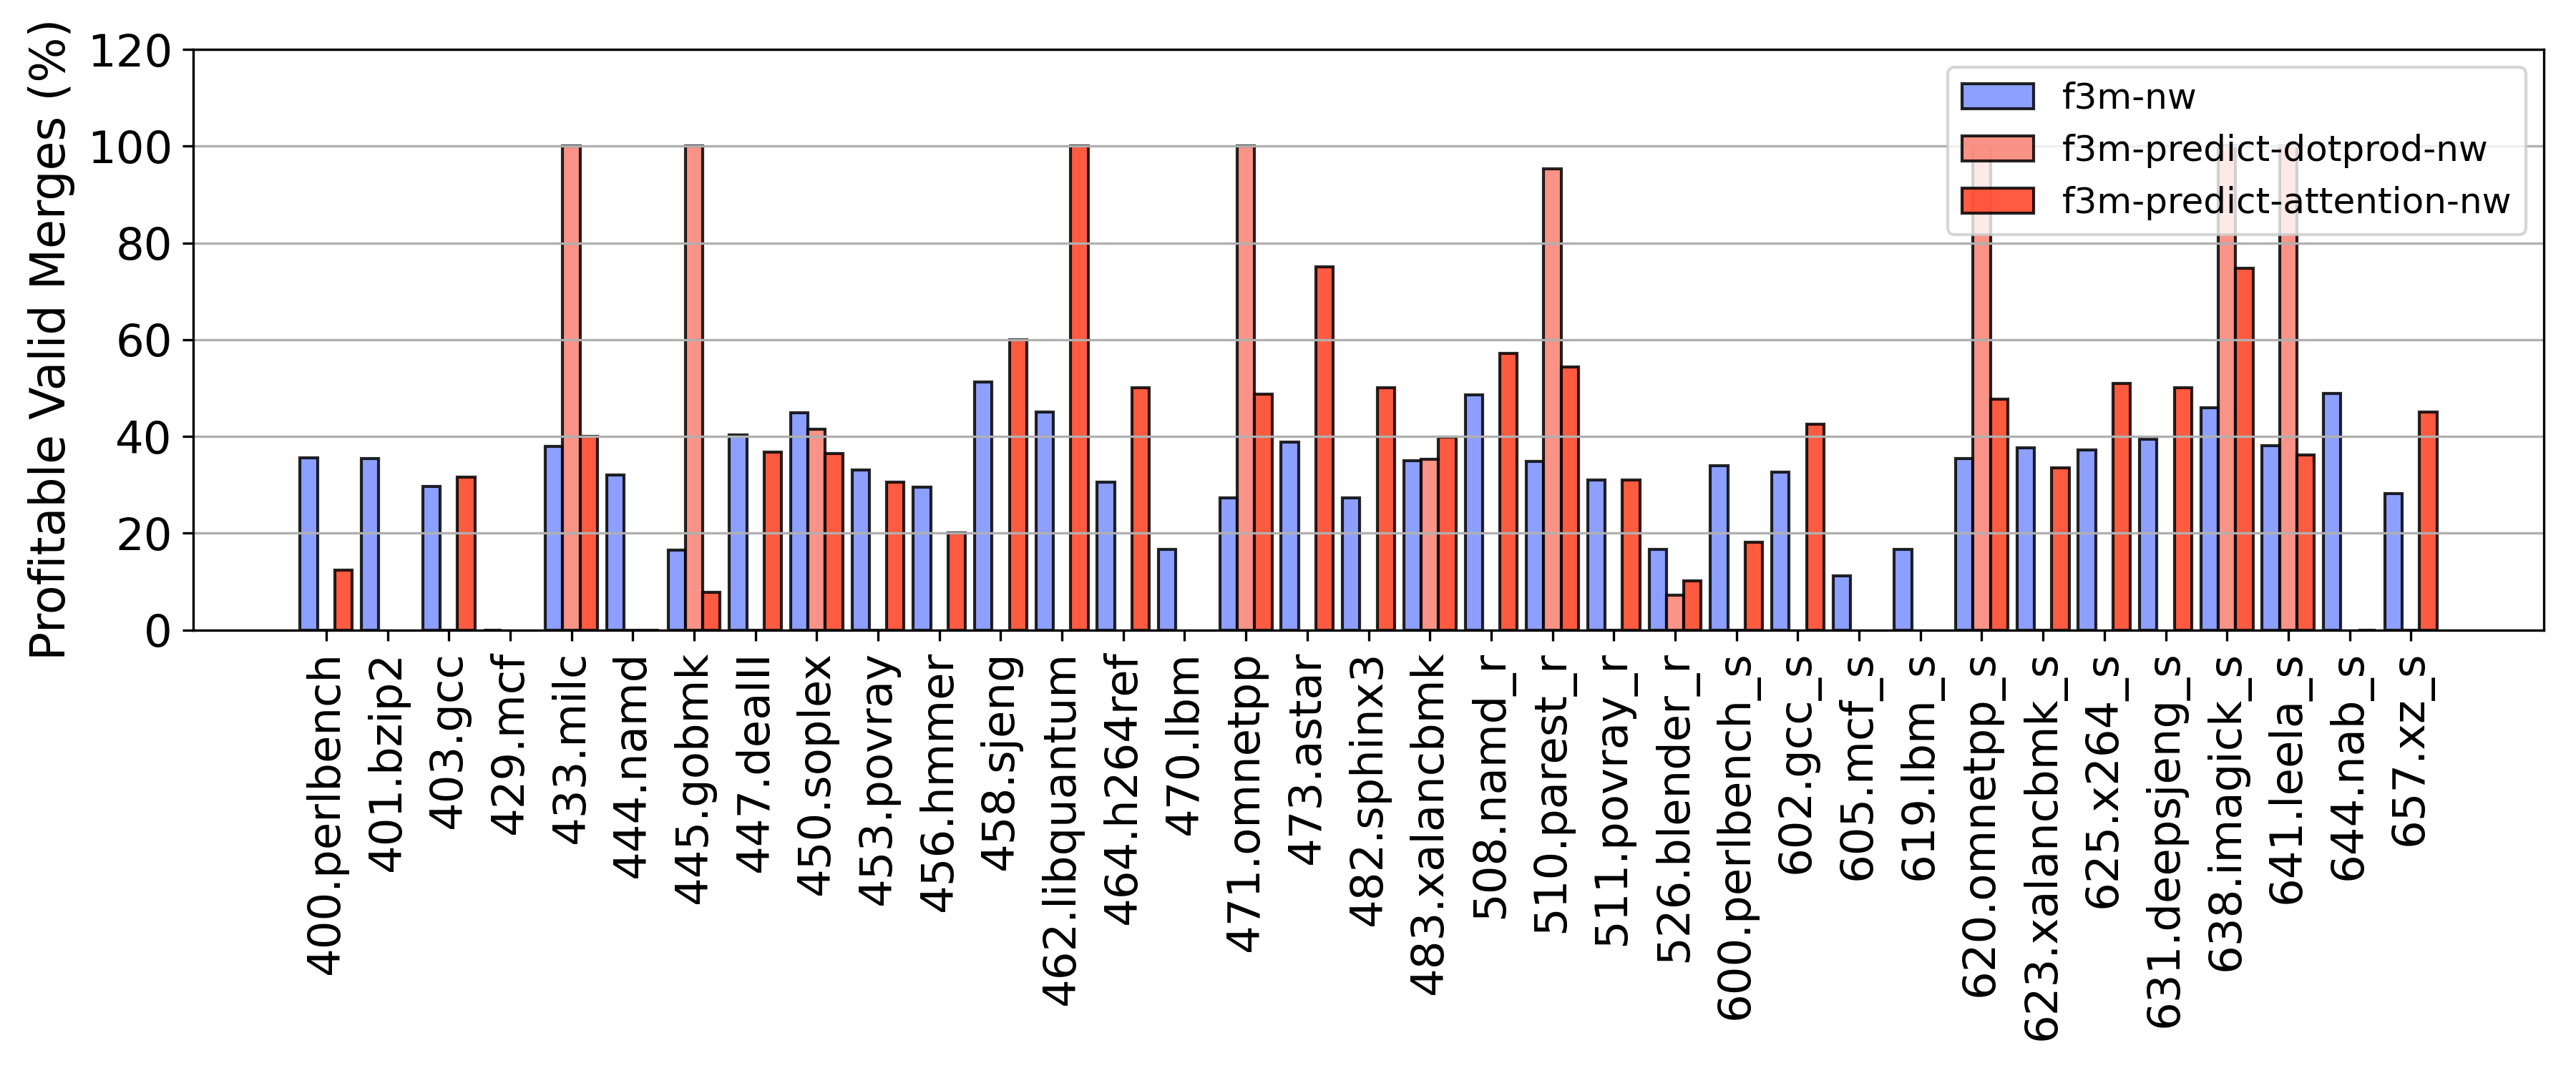
\includegraphics[scale=0.47]{Figures/Valid_Merging_Predictions/0.5_ValidProfitablePercentage.png}
        \caption{\textbf{Profitable Valid Merges (\textbf{0.5} Threshold)}} 
        \label{fig:0.5ValidProfitable}
    \end{subfigure}
    \begin{subfigure}{\textwidth}
    \centering
        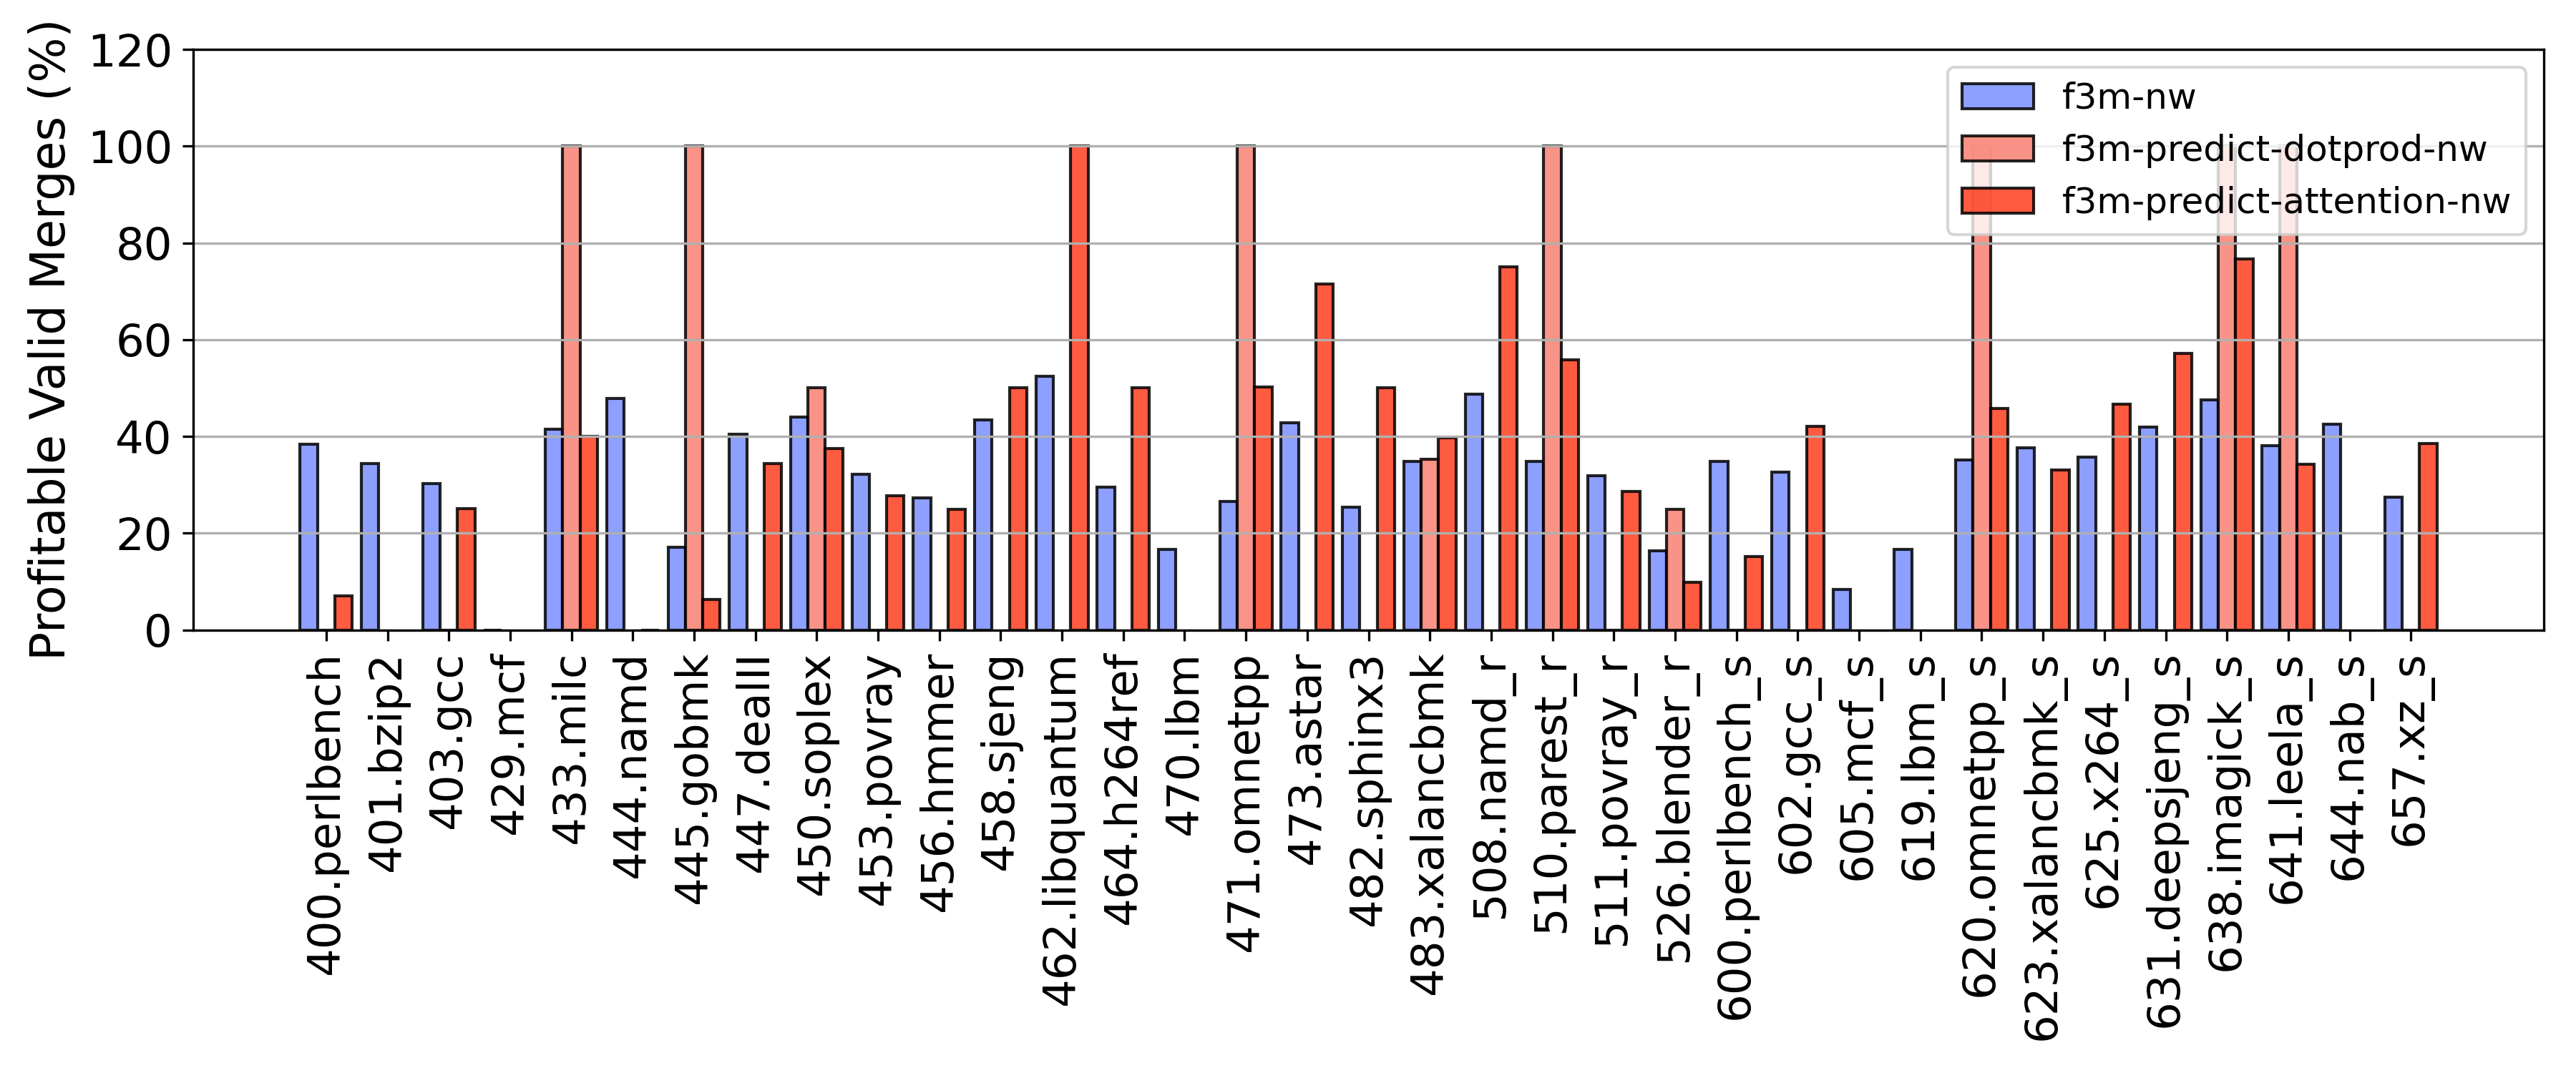
\includegraphics[scale=0.47]{Figures/Valid_Merging_Predictions/0.6_ValidProfitablePercentage.png}
        \caption{\textbf{Profitable Valid Merges (\textbf{0.6} Threshold)}} 
        \label{fig:0.6ValidProfitable}
    \end{subfigure}

    \caption{\textbf{Percentage of Valid Merges that are Profitable.} This graph illustrates the proportion of valid merges that result in code size reduction, calculated using equation \ref{METRIC:ValidProfitablePercentage}.} 
    \label{fig:ValidProfitable}
\end{figure}


When comparing the performance of our different approaches across benchmarks, the prediction-based approaches generally outperform the baseline F3M across most benchmarks, with these performance differences remaining fairly consistent across all thresholds. However, exceptions exist, particularly with benchmark 401.bzip2, where the baseline outperforms both prediction models in all thresholding.

The dot product model exhibits the most distinctive behaviour, showing the highest peaks on several benchmarks reaching 100\% profitable valid merges. Yet this approach demonstrates considerable instability, oscillating between exceptional and poor performance with few benchmarks exhibiting moderate results. Most importantly, these impressive profitability percentages must be interpreted with caution due to the dot product model's significantly lower valid function merge count. When a model finds very few valid merges to begin with, even if most of them are profitable, the absolute benefit may be minimal compared to approaches that find more valid merge candidates.
In contrast, the attention model shows a more consistent and reliable pattern. It produces more profitable merges compared to F3M regardless of threshold, also achieving 100\% valid-profitability rates in certain phases, but crucially maintains a higher count of valid function merges. This balance makes the attention model more practical, as it wastes less computational resources by identifying a substantial number of merge opportunities while still maintaining high profitability rates.

\subsection{Evaluation}
The Dot Product Model demonstrates significant limitations as a heuristic for function merging. Despite occasionally proposing more merges than F3M at a 0.4 threshold and matching its volume at 0.5, its precision remains unacceptably low, topping out at only 29\% valid merges on the 433.milc benchmark at a 0.6 threshold. This indicates that over 70\% of its attempted merges are invalid and cannot produce merge-able function pairs, representing substantial wasted computational effort during compilation. Although the model reports a deceptively high profitable‑to‑valid ratio, this metric is undermined by an exceedingly small pool of valid candidates rather than by robust predictive power, rendering it an unreliable indicator of overall effectiveness for the model's performance.

The Attention Model presents a more conservative approach than F3M, generating significantly fewer merge attempts than F3M, sometimes less than half as many. This reduction raises two possible interpretations, either the model fails to identify viable merging opportunities that F3M captures or achieves superior global optimisation by prioritising the most beneficial merges first, leaving fewer similar functions available for subsequent merges. This progressive improvement in validity suggests that higher thresholds effectively filter out invalid merge candidates at the expense of the volume of merging attempts.

When profitability is considered, the Attention Model maintains consistent performance across all tested thresholds when measuring the ratio of attempted merges that yield profitable outcomes (17/35 benchmarks matching or exceeding F3M at every threshold), underscoring its stable precision across score cut‑offs. However, the proportion of valid merges that are profitable exhibits an inverse relationship with the threshold, performing best at 0.4 (20/35 benchmarks) and declining at higher thresholds (14/35 at 0.6). This suggests that while higher thresholds improve validity prediction, they may be overly conservative in identifying profitable merging opportunities, potentially excluding borderline cases that could yield modest but worthwhile code size reductions. In practice, a balance must be struck between the ratio of merging validity and valid-profitable merges by tuning the threshold.

The evidence indicates that the Attention Model substantially outperforms the Dot Product Model as a function merging heuristic. Despite its high proposal volume, the Dot Product approach suffers from a poor invalid merge rate (over 70\%).In contrast, the Attention Model delivers a noticeably better balance of validity and profitability, particularly around a 0.5 threshold, where it matches or exceeds F3M's performance. Although its conservative proposal strategy may miss merge opportunities that F3M identifies, this could reflect a more globally optimal merge ordering rather than the omission of opportunities. Further evaluation is needed to determine whether the Attention Model's reduced attempt count represents optimality or overlooks merges.

While both prediction models demonstrate superior precision in selecting profitable merging candidates when they succeed in finding valid pairs, the attention model's combination of reasonable valid merge counts and high profitability makes it the more promising approach for real-world compiler optimisation scenarios.


\todo{Choose 0.5 seems to be the best, because it is able to balance the number }
\todo{Mention that mcf is quite small, so functionmerging is not done for most of it. So should consider a total of 34 instead of 35 benchmarks???}


\todo{Attention Model does not seem to be able to pick out options from a small pool of functions, it tensds to work better when given a large pool of functions: Validity}.


\section{Code Size Reduction}
Lastly, we analyse the effect the three different approaches for function merging: F3M, Dot Product Predictions and Attention Predictions, have on code size reduction when compared to a LLVM's default compiled binary without aggressive function merging. There are two metrics this evaluation focuses on, the \textbf{\textit{.text size}} and the \textbf{\textit{binary size}}. The .text section of an executable contains only the actual machine code instructions, holding the compiled code that will be executed at runtime. The binary size, on the other hand, refers to the total size of the compiled file, this includes all the machine code instructions, global variables, read-only data, and other metadata specific to the executable format. The .text section size provides direct insight into the effectiveness of function merging optimisation, while the binary size allows us to understand the overall impact on the executable size.

Since F3M employs heuristics with randomised components, it is not deterministic. To account for this variability, it was executed three times and the average was taken for the results. The deep learning approach, which predicts alignment scores between function pairs using IR2Vec embeddings, aims to achieve better code size reduction than F3M.

\subsection{.text Size Reduction}
Figures \ref{fig:DotTextSizeComparison}, presents the .text section size reduction achieved by our three function merging approaches (F3M, Dot Product Predictions, and Attention Predictions) across the benchmark suite compared to the baseline LLVM compilation. The .text section size reduction directly measures each approach's effectiveness at eliminating redundant code through function merging, with higher percentages indicating more successful optimisation. This metric is particularly relevant as it isolates the impact on actual executable code size, allowing us to evaluate each method's capability to identify and merge similar functions while excluding other factors that may affect overall binary size.


\begin{figure}[tbh!]
    \centering
    \begin{subfigure}{\textwidth}
        \centering
        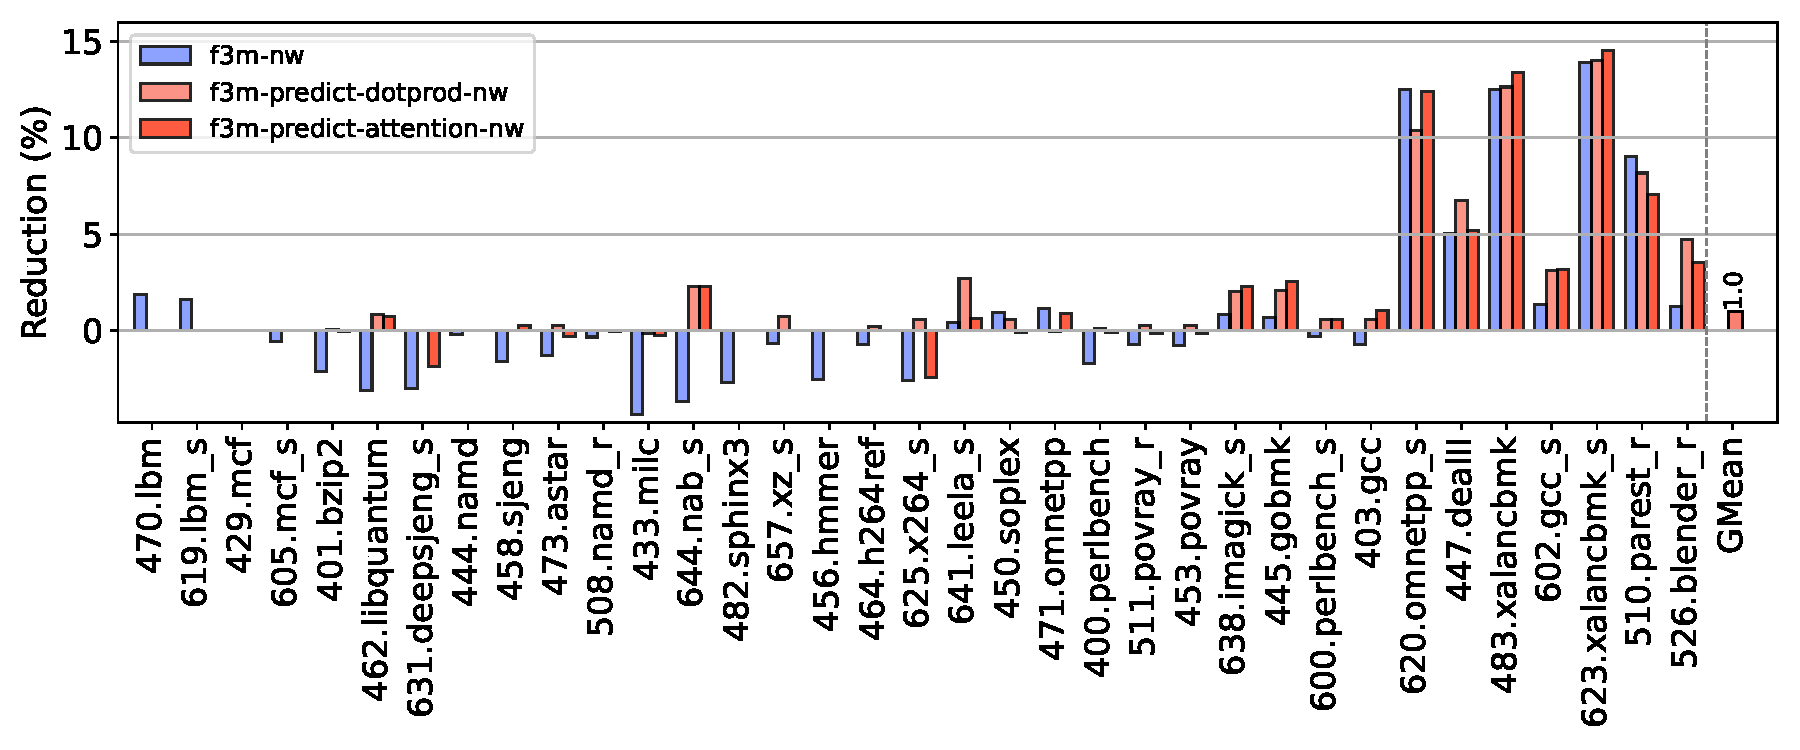
\includegraphics[scale=0.47]{Figures/CodeSizeAnalysis/0.4_dottext_code-size-reduction.pdf}
        \caption{Dot Text Size Reduction with \textbf{0.4} Threshold)}
        \label{fig:0.4BinSizeCodeSize}
    \end{subfigure}
    \begin{subfigure}{\textwidth}
        \centering
        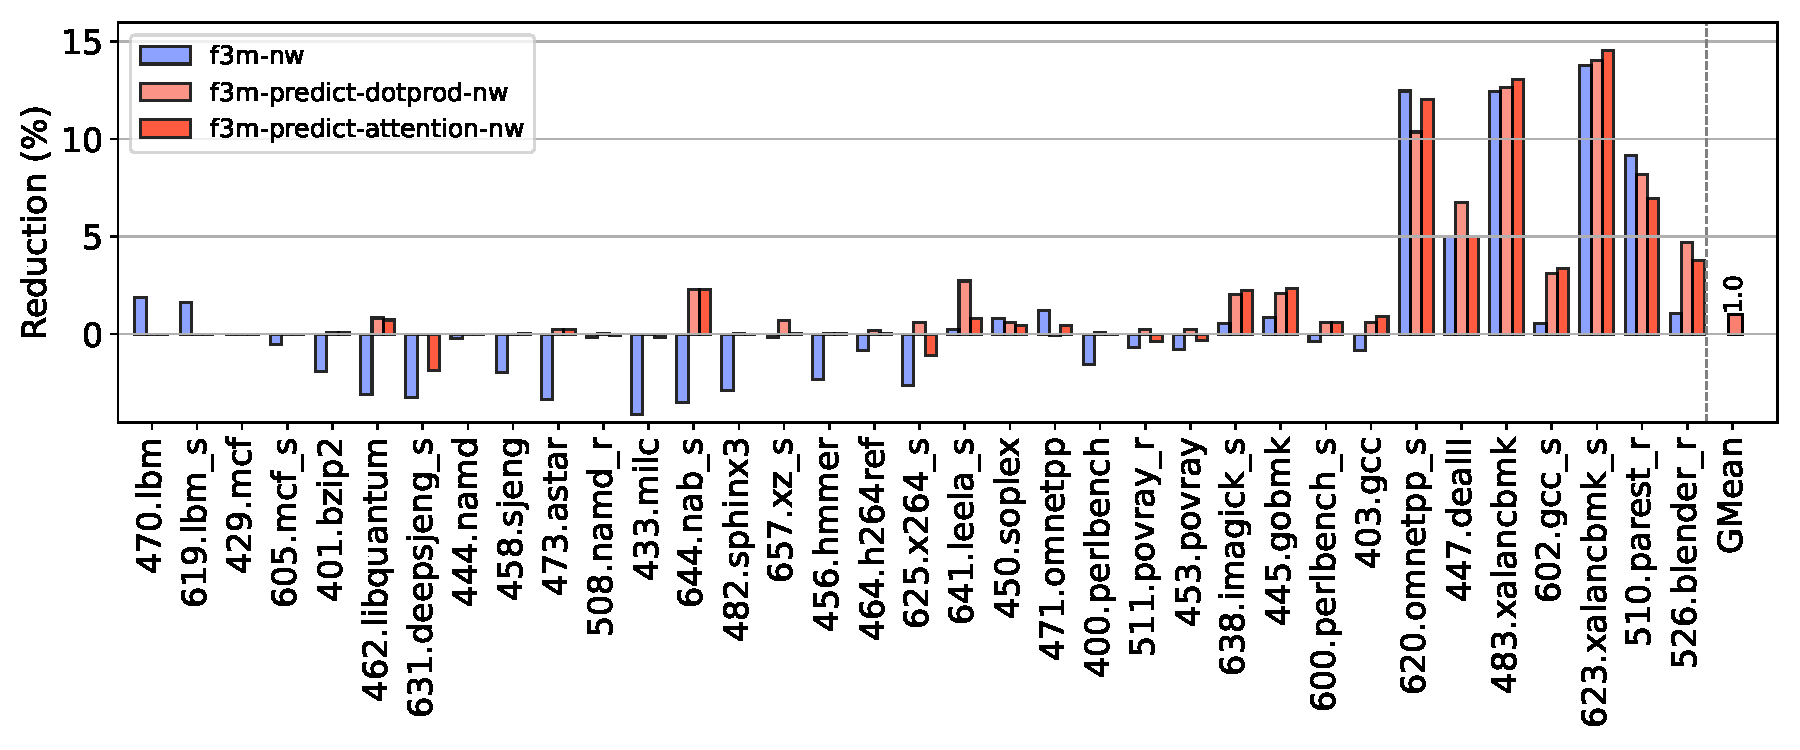
\includegraphics[scale=0.47]{Figures/CodeSizeAnalysis/0.5_dottext_code-size-reduction.pdf}
        \caption{Dot Text Size Reduction with \textbf{0.5} Threshold)}
        \label{fig:0.5BinSizeCodeSize}
    \end{subfigure}
    \begin{subfigure}{\textwidth}
    \centering
        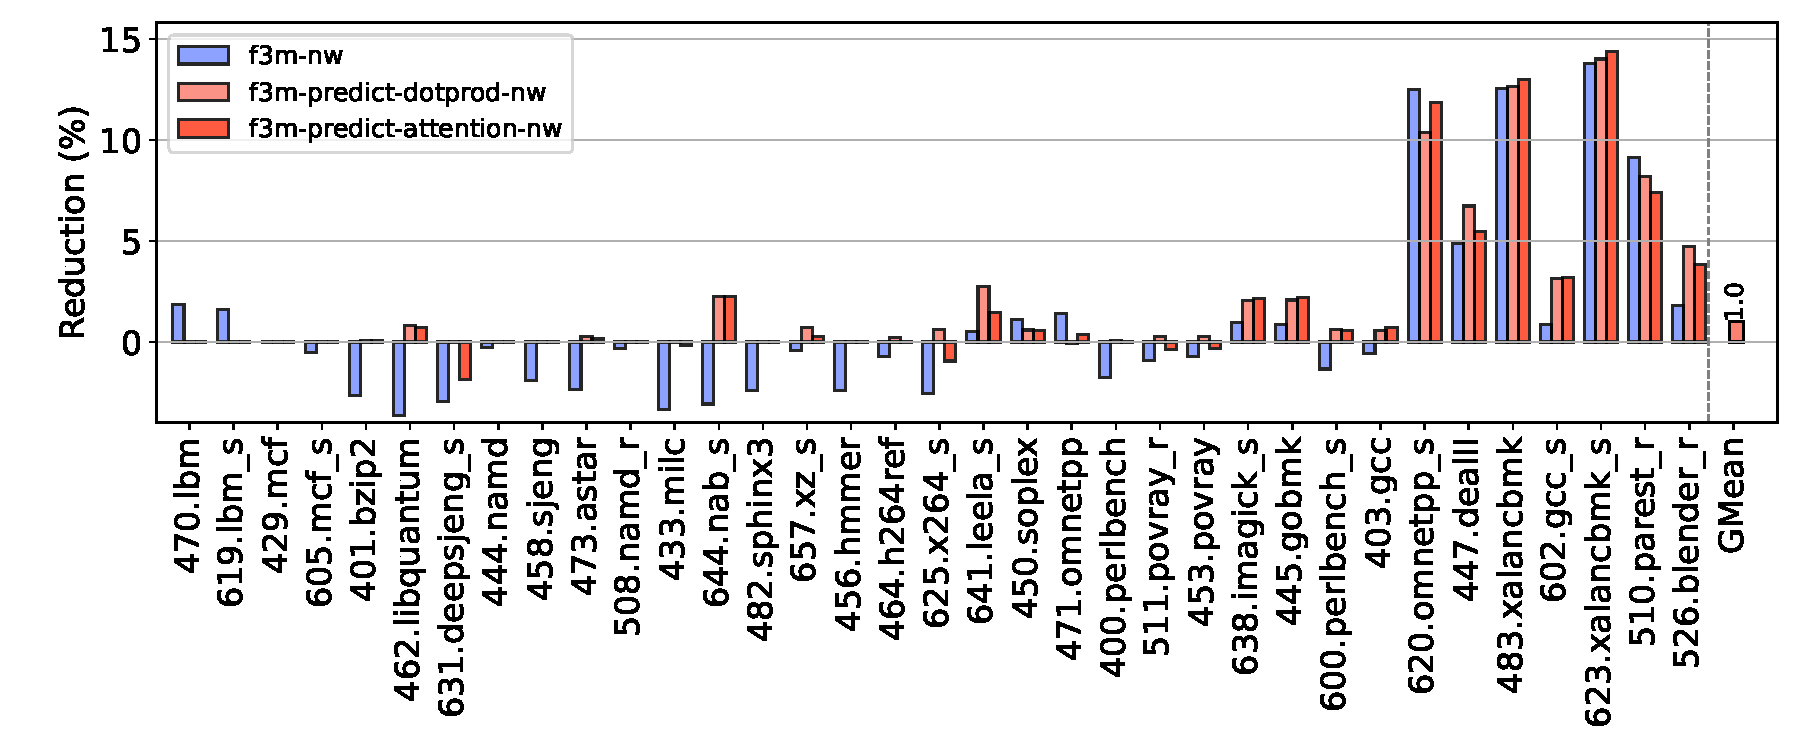
\includegraphics[scale=0.47]{Figures/CodeSizeAnalysis/0.6_dottext_code-size-reduction.pdf}
        \caption{Dot Text Size Reduction with \textbf{0.6} Threshold)}
        \label{fig:0.6BinSizeCodeSize}
    \end{subfigure}

    \caption{\textbf{Dot Text Size Reductions Across Different Thresholds.} The percentage of dot text size reduction is shown against the baseline, which is the default LLVM without any experimental function merging (Higher is better).}
\label{fig:DotTextSizeComparison}
\end{figure}

F3M achieved an average .text size reduction of \textbf{2.9}\% across SPEC2006 and SPEC2017 benchmarks, while our machine learning-based approaches demonstrated superior performance with reductions of \textbf{4.4}\% and \textbf{4.2}\% for the Dot Product and Attention models respectively. This represents a significant improvement of approximately 50\% over the state-of-the-art F3M technique.

While examining individual benchmark performance, F3M outperformed our predictive models on four benchmarks (450.soplex, 471.omnetpp, 620.omnetpp\_s, and 510.parest\_r) consistently across all threshold configurations. However, our predictive approaches demonstrated greater consistency at reducing the .text size, particularly on smaller benchmarks where F3M frequently increased the .text size rather than reducing it.

Regarding threshold sensitivity, the Dot Product model showed identical performance at thresholds of 0.5 and 0.6, with minimal difference when lowered to 0.4, suggesting that the higher 0.6 threshold could be preferred to reduce computational overhead. The Attention model exhibited even more stable behaviour, with reduction percentages ranging narrowly from 4.24\% to 4.29\% across different thresholds. This shows that the threshold does not play a big role in the .text's size. This stability indicates that the threshold selection does not play a big role in the .text size reduction effectiveness at the granularity of thresholds we assessed.

Both the Dot Product and Attention model significantly surpassed F3M's capabilities, demonstrating that our machine learning approach successfully captures function similarities that traditional heuristic-based methods miss.

In summary, both the Dot Product and Attention model frequently surpassed F3M's capabilities, demonstrating that our machine learning approach successfully captures function similarities that traditional heuristic-based methods miss.

\subsection{Binary Size Reduction}
While .text size reduction focusses on executable code sections, binary size reduction provides a more comprehensive view of optimisation impact, capturing potential overheads in metadata, branch tables, and other sections that might be introduced during function merging. This metric is important for evaluating real-world deployment scenarios where total storage requirements matter, particularly in resource-constrained environments like embedded systems or mobile applications. Figures \ref{fig:binSizeComparison} shows the overall binary size reduction achieved by our three function merging approaches (F3M, Dot Product Predictions, and Attention Predictions) across Spec2006 and Spec2017 benchmarks compared to the baseline default LLVM compilation. 

\begin{figure}[tbh!]
    \centering
    \begin{subfigure}{\textwidth}
        \centering
        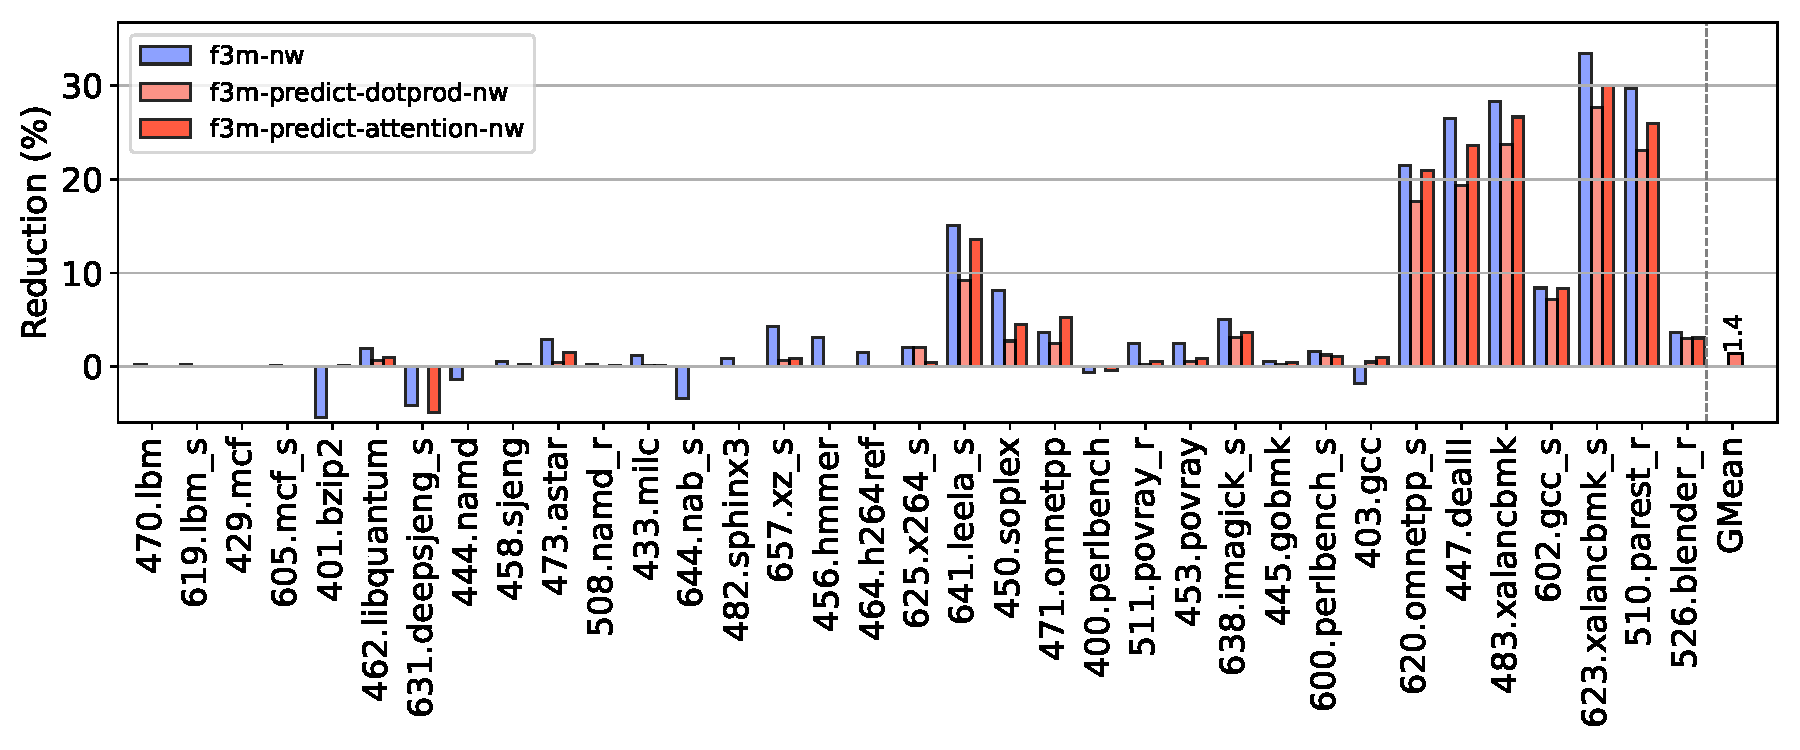
\includegraphics[scale=0.47]{Figures/CodeSizeAnalysis/0.4_binsize_code-size-reduction.pdf}
        \caption{\textbf{Binary Size Reduction (\textbf{0.4} Threshold)}} 
        \label{fig:0.4BinSizeCodeSize}
    \end{subfigure}
    \begin{subfigure}{\textwidth}
        \centering
        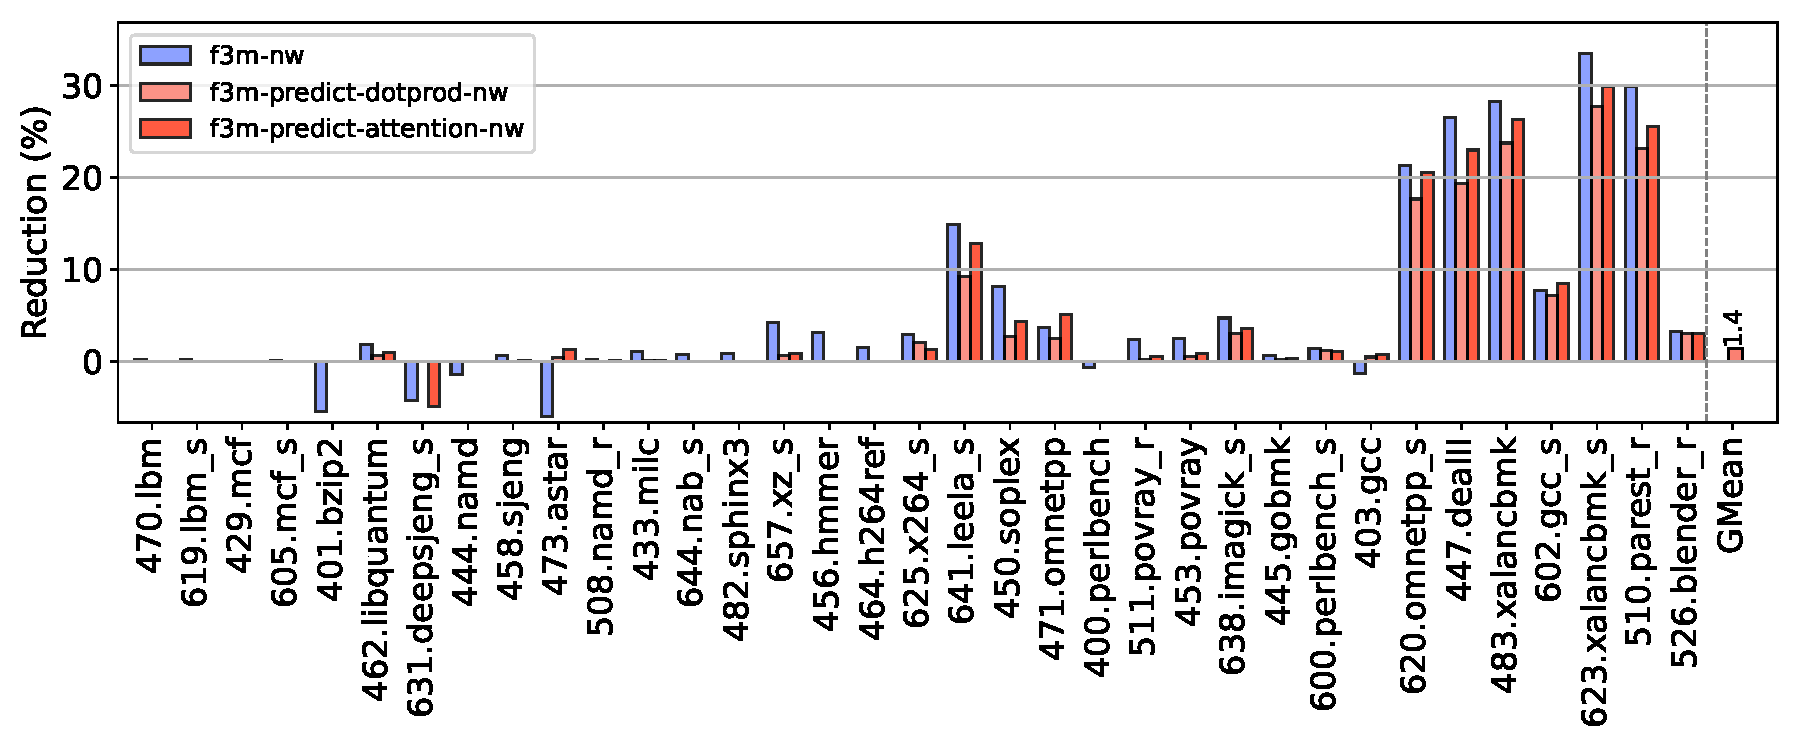
\includegraphics[scale=0.47]{Figures/CodeSizeAnalysis/0.5_binsize_code-size-reduction.pdf}
        \caption{\textbf{Binary Size Reduction (\textbf{0.5} Threshold)}} 
        \label{fig:0.5BinSizeCodeSize}
    \end{subfigure}
    \begin{subfigure}{\textwidth}
    \centering
        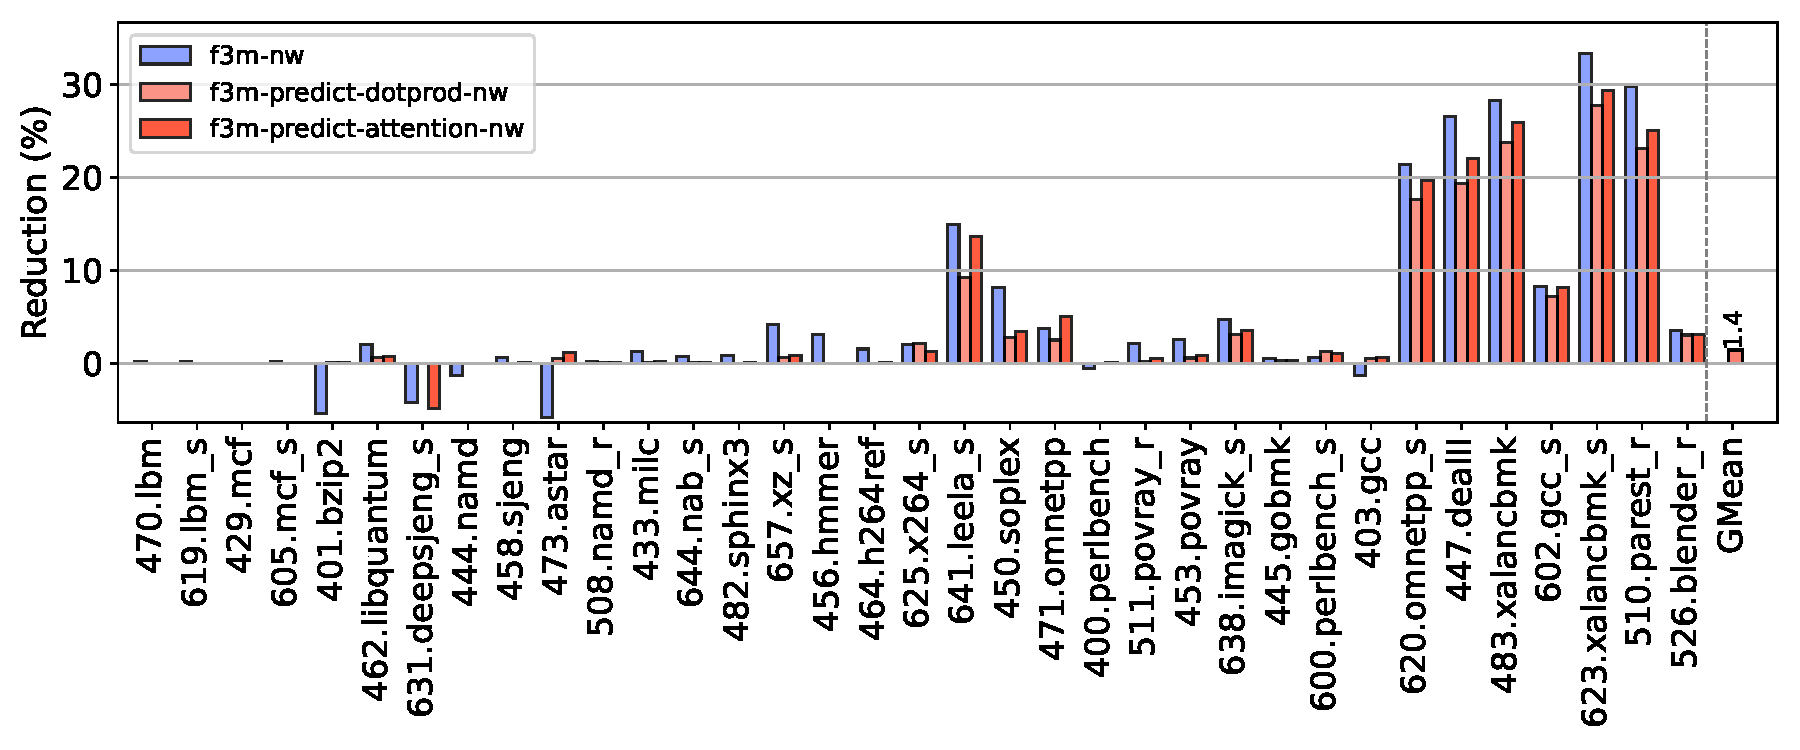
\includegraphics[scale=0.47]{Figures/CodeSizeAnalysis/0.6_binsize_code-size-reduction.pdf}
        \caption{\textbf{Binary Size Reduction (\textbf{0.6} Threshold)}} 
        \label{fig:0.6BinSizeCodeSize}
    \end{subfigure}

    \caption{\textbf{Binary Size Reductions Across Different Thresholds.} The percentage of binary size reduction is shown against the baseline, which is the default LLVM without any experimental function merging (Higher is better).}
\label{fig:binSizeComparison}
    \label{fig:binSizeComparison}
\end{figure}

Unlike the .text size results, figure \ref{fig:binSizeComparison} reveals the traditional F3M approach maintains an edge in overall binary optimization, achieving a substantial \textbf{12.1\%} reduction across our benchmark suite. Our machine learning techniques demonstrated respectable but lesser reductions of \textbf{9.9\%} (Dot Product) and \textbf{11\%} (Attention), suggesting F3M's heuristics may better address factors beyond code sections that influence total executable size. The Attention model was able to show promising results on three benchmarks (\textit{471.omnetpp}, \textit{403.gcc}, and \textit{602.gcc\_s}), where it outperformed F3M across all threshold configurations.

The predictability of our ML-based approaches stands as their most compelling advantage. The Dot Product model exhibited remarkable consistency, producing zero negative outcomes across all benchmarks, a guarantee against unwanted size increases that F3M cannot provide. Similarly, the Attention model triggered negative reduction in just one case (\textit{631.deepsjeng\_s}), vastly outperforming F3M's unpredictable behaviour on smaller benchmarks, while F3M increased binary size on multiple smaller benchmarks, making our approaches more reliable for size-sensitive applications.

Threshold configuration analysis revealed minimal sensitivity across both models. The Attention implementation showed slightly better performance at lower thresholds (ranging from 10.7\% to 11.1\% reduction), but the practical difference remains negligible for most deployment considerations. The Dot Product model's results at 0.4, 0.5 and 0.6 thresholds are almost identical, further emphasising this stability.

\subsection{Evaluation}
% Finally, both metrics are examined together, to better understand how effectively machine learning can be utilised to eliminate redundant code and how it manages the broader implications of function transformations on the complete executable.

% It seems that none of the implementations were able to make a break through with MCF, no matter the threshold as well, probably because there isn't enough functions to choose from.


% Dot product seems to do pretty well despite its poor merging prediction quality. So dot product is working a bit like f3m in this case where it helps shortlist functions for the compiler to try to merge?

% If we look at the .text size reduction, the predictive approach managed to work better than F3M (4.3\% vs 2.9\% reduction on baseline), showing a 48\% improvement. This is the metric which best shows the effects that function merging has on the code and it shows that this is showing superior performance compared to the previous state of the art, showing that this is a really significant improvement, for both predictive models.

% While the predictive models work quite well, even with its ability to decrease the binary size by 10.5\%, it falls slightly behind F3M (12.1\%), a 13.2\% decrease in reduction compared to F3M. But consider that this reduction came without any heuristic used to decide the function merges.

% The reason that this is happening is because of the data stored for exception handling. The exception handling frame is used to ... . And the exception handling frame header is used for ... . The exception handling frame for the dor product and attention models are 13.6\% and 8.5\% larger than F3M's and is 11.7\% and 6.9\% larger for the  the exception handling frame header.
% \todo{Check to see if this information is correct}


% One reason for this could be attributed to the data stored for exception handling. The exception handling frame (\textbf{.eh\_frame} section) is used to store the \textit{call frame information} which describes how to restore the stack state at any point in program execution, necessary for stack unwinding during exception propagation. The exception handling frame header (\textbf{.eh\_frame\_hdr} section) is used for binary searching into the exception handling frame during runtime to quickly locate the appropriate frame description entry for a given program counter value, working as an optimisation to make exception handling more efficient.

% When functions are merged, the CFI must maintain precise stack unwinding instructions for each possible execution path through the merged function. This requires additional CFI directives to track stack unwinding information across multiple execution paths that previously existed in separate functions. The merged function must maintain all exception-handling capabilities of the original functions while now managing them within a single code body, leading to a substantial increase in exception metadata despite the reduction in code size.

% The exception handling frame for the dot product and attention models are 13.6\% and 8.5\% larger than F3M's and is 11.7\% and 6.9\% larger for the exception handling frame header. This demonstrates how function merging can lead to smaller .text sections but larger overall binaries due to this metadata expansion.

% If users are willing to take a slight risk when running function merging, it is better to use attention model than dot product, because the size will likely be smaller if the code size is reduced, but there is a small chance that the size will increase slightly.

% There is also performance left on the table since the merged functions were not taken into consideration for merging again due to IR2Vec's versioning issues described in \ref{Design:IntegratingLLVM}.

% On the other hand, dot product is safer, much less likely to generate a larger size, for both the .text and binary size but the reduction is less aggressive.

% The compile time for the dot product approach and the attention model approaches are 10 and 23 times the time it takes for F3M. The reason that the predictive models are a multitude larger than F3M, this is due to the way it was implemented where the alignment score is generated between a function and all other functions, before being merged with the highest aligned function. This process is costly, and it could benefit from a multi-tiered analysis process where earlier stages will prune off non-profitable functions to predict scores for since most function pairs do not align well. Simplifying the process and wasting less computational power on running the compiler.

% ===========

It seems that none of the implementations were able to make a breakthrough with both mcf benchmarks, regardless of threshold, likely because there aren't enough functions to choose from. Despite this limitation, both predictive models showed promising results when examining how effectively machine learning can eliminate redundant code while managing the broader implications of function transformations on the complete executable.

If we look at the \textit{.text} size reduction, the predictive approach managed to work better than F3M (4.3\% vs 2.9\% reduction on baseline), showing a 48\% improvement. This metric best demonstrates the effects of function merging on code and indicates superior performance compared to the previous state of the art, representing a significant improvement for both predictive models. Surprisingly, the dot product approach performs well despite its poor merging prediction quality, functioning similarly to F3M by helping shortlist functions for the compiler to attempt merges on.

While the predictive models work quite well, with its ability to decrease binary size by 10.5\%, but they fall slightly behind F3M (12.1\%), representing a 13.2\% decrease in reduction performance compared to F3M, but do keep it in mind that this reduction was achieved without any heuristic used to decide the function merges.

One reason for this discrepancy can be attributed to the data stored for exception handling. The exception handling frame (.eh\_frame section) is used to store the call frame information (CFI) which describes how to restore the stack state at any point in program execution, necessary for stack unwinding during exception propagation. The exception handling frame header (.eh\_frame\_hdr section) is used for binary searching into the exception handling frame during runtime to quickly locate the appropriate frame description entry for a given program counter value, working as an optimisation to make exception handling more efficient.

When functions are merged, the CFI must maintain precise stack unwinding instructions for each possible execution path through the merged function. This requires additional CFI directives to track stack unwinding information across multiple execution paths that previously existed in separate functions. The merged function must maintain all exception-handling capabilities of the original functions while now managing them within a single code body, leading to a substantial increase in exception metadata despite the reduction in code size.

The exception handling frame for the dot product and attention models are 13.6\% and 8.5\% larger than F3M's and is 11.7\% and 6.9\% larger for the exception handling frame header. This demonstrates how function merging can lead to smaller \textit{.text} sections but larger overall binaries due to this metadata expansion.

If users are willing to take a slight risk when running function merging, it is better to use the attention model than dot product, because the binary size will likely be smaller if the code size is reduced, though there is a slight chance that the size will increase slightly. On the other hand, dot product is safer, much less likely to generate a larger size for both the .text and binary size, but the reduction is less aggressive.

There is also performance left on the table since the merged functions were not taken into consideration for merging again due to IR2Vec's versioning issues. The compile time for the dot product approach and the attention model approaches are 10 and 23 times longer than F3M respectively. This is due to the implementation where the alignment score is generated between a function and all other functions before merging with the highest aligned function. This process is costly and could benefit from a multi-tiered analysis process where earlier stages prune off non-profitable functions, simplifying the process and wasting less computational power on running the compiler.